% !TEX program = pdflatex
% Evidence-led staging draft. Statistics, Results, Discussion and Conclusions
% are deliberately outside this version.

\documentclass[12pt,a4paper]{article}

\usepackage[margin=2.5cm]{geometry}
\usepackage{graphicx,booktabs,array,amsmath,siunitx,natbib,caption,subcaption,placeins,setspace,lineno,url,rotating}
\usepackage[hidelinks]{hyperref}

\graphicspath{{../figures/}}
\sisetup{separate-uncertainty=true,per-mode=symbol,range-phrase={--},range-units=single}
\onehalfspacing
\linenumbers

\title{Spatio-temporal heterogeneity of gas concentrations and its propagation into ventilation and emission estimates in a naturally ventilated dairy barn}
\author{Harsh Sahu$^{a,b}$, Long Chen$^{a}$, Thomas Amon$^{a,b}$, David Janke$^{a,*}$}
\date{}

\begin{document}
\maketitle
\begin{center}\small
$^{a}$Leibniz Institute for Agricultural Engineering and Bioeconomy (ATB), Max-Eyth-Allee 100, 14469 Potsdam, Germany\\
$^{b}$Institute of Animal Hygiene and Environmental Health, Department of Veterinary Medicine, Freie Universit\"at Berlin, Germany\\
$^{*}$Corresponding author: \href{mailto:djanke@atb-potsdam.de}{djanke@atb-potsdam.de}
\end{center}

\section{Introduction}

Dairy housing is an important source of methane (\(\mathrm{CH_4}\)) and ammonia (\(\mathrm{NH_3}\)), and reliable barn-scale measurements are needed to evaluate mitigation measures and compile emission inventories. Naturally ventilated dairy barns are widely used because large wall and ridge openings provide fresh air without the continuous energy demand of mechanically driven ventilation. The same openness makes these buildings unusually difficult measurement systems. Wind direction and speed, buoyancy, roof geometry, animals, manure surfaces and internal obstructions continuously redistribute both air and gases. Openings can alternate between inlet and outlet behaviour, and the concentration sampled at one position may therefore not represent either the average barn air or the air mass carrying pollutants out of the building \citep{Calvet2013,Ogink2013,Saha2013}.

This spatial problem affects direct and indirect emission methods differently but cannot be avoided by either. Direct methods require concentration and velocity to be resolved over the effective outlet area. In a scaled naturally ventilated building, a constant-height concentration configuration produced emission errors as large as 97\%, whereas vertically resolved concentration sampling reduced the error to below 5\% for the investigated cases \citep{Janke2020}. Indirect tracer or \(\mathrm{CO_2}\)-balance methods avoid direct integration of opening velocity, but they require representative indoor and outdoor concentrations. Error in the indoor \(\mathrm{CO_2}\) concentration propagates into the calculated ventilation rate, and spatial error in the pollutant concentration subsequently propagates into the calculated emission. Consequently, analytical accuracy and calibration are necessary but insufficient: the sampled air must also be spatially representative.

Previous work has examined complementary parts of this problem. Opening- and wind-oriented field studies showed that external wind and the selection of indoor and outdoor sampling positions affected measured concentrations, air exchange and calculated emissions \citep{Saha2013,Koenig2018,JankeSampling2020}. Horizontal mapping in an open-sided dairy barn used 11 locations at 0.2 m above the floor and showed that location, number and spacing influenced the estimated concentrations; the authors compared one-, two- and three-location subsets with four-location area means using one-way analysis of variance and Tukey comparisons \citep{Durso2022}. In a naturally ventilated animal mock-up, De Vogeleer et al. demonstrated that the spatial arrangement of sampling points could be as consequential as their number, although transfer from an unoccupied mock-up to a full-scale barn with biological heat and gas sources remains uncertain \citep{DeVogeleer2017}. These studies establish that horizontal replication matters, but they do not describe a barn-wide three-dimensional concentration field.

Vertical studies likewise show that one universal sampling height cannot be assumed. Mendes et al. sampled \(\mathrm{NH_3}\), metabolically produced \(\mathrm{CO_2}\) and injected \(\mathrm{SF_6}\) at 1, 2, 3 and 4 m near an inlet and an outlet. Two-way analysis of variance followed by Tukey--Kramer comparisons indicated that concentrations and pollutant-to-tracer ratios became more stable above the animal-occupied zone under the tested conditions \citep{Mendes2015}. D'Urso et al. measured \(\mathrm{NH_3}\), \(\mathrm{CH_4}\) and \(\mathrm{CO_2}\) at three heights in an open Mediterranean barn and used one-way analysis of variance, Tukey comparisons, Pearson correlations and regressions to demonstrate gas-specific vertical behaviour \citep{Durso2024}. At a building outlet, Sahu et al. found significant concentration gradients across vertically distributed sampling points \citep{Sahu2023}. Conversely, a parametric CFD study showed that the commonly recommended height of at least 3 m only rarely coincided with a perfect pollutant-to-tracer mixing ratio; the most representative height depended on convection regime and inflow direction \citep{Doumbia2021}. Thus, a convenient height may be representative for one gas or flow regime without being representative for another.

Measurements close to animals address a different spatial scale. Wu et al. placed nine sampling locations at 0.3 m around two lying cubicles and a barn-background location at 3.5 m. Hourly \(\mathrm{CH_4}\) concentrations around the cubicles had spatial coefficients of variation of 71\% in summer and 58\% in winter, while temporal coefficients of variation were still larger at several locations; airflow, cow occupancy and barn management were identified as important drivers \citep{Wu2016}. Airflow and \(\mathrm{CO_2}\) measurements at 1.5 and 2.6 m also showed that only part of a windward opening necessarily benefited from the approaching wind and that the association between wind speed and \(\mathrm{CO_2}\) was not adequately represented by a simple linear relationship \citep{Fiedler2014}. Near-source studies are therefore indispensable for understanding animal and manure microenvironments, but they answer a different question from whether the accessible upper barn airspace provides a representative concentration for whole-building measurements.

Gas ratios provide an additional test of spatial coherence. If two gases experience identical source-to-sensor transport and dilution, their ratio should be more stable than either concentration alone. Mendes et al. showed that stable ratios can occur even when the individual gases are not homogeneously distributed, provided that pollutant and tracer dispersion patterns remain sufficiently similar \citep{Mendes2015}. However, \(\mathrm{CO_2}\), \(\mathrm{CH_4}\) and \(\mathrm{NH_3}\) have overlapping but non-identical sources and removal processes. Respiration and enteric release are coupled to animal position and activity, whereas \(\mathrm{NH_3}\) is strongly affected by manure surfaces, temperature, air movement and deposition. Spatial variation in \(\mathrm{NH_3}/\mathrm{CO_2}\), \(\mathrm{CH_4}/\mathrm{CO_2}\) or \(\mathrm{NH_3}/\mathrm{CH_4}\) can therefore reveal divergence that is concealed by common ventilation-driven concentration changes.

The existing literature is consequently rich but spatially fragmented. Studies have concentrated on particular openings, horizontal transects, a small number of vertical levels, near-cubicle microenvironments, sampling-line strategies, mock-ups or numerical flow fields. Dense measurements combining extensive horizontal coverage, conventional upper-air sampling and uncommon near-roof positions over an occupied barn and changing seasonal conditions remain scarce.

The aim of this study was to characterise the spatial structure of \(\mathrm{CO_2}\), \(\mathrm{CH_4}\), \(\mathrm{NH_3}\) and their ratios inside a naturally ventilated dairy barn using 51 sampling points arranged as 17 horizontal positions and three vertical levels. The hypothesis was that gas concentrations and gas ratios exhibit systematic spatial structure with sampling height and horizontal position inside the barn. Consequences of spatial coverage, vertical coverage, density and temporal aggregation for representative concentrations and indirect \(\mathrm{CO_2}\)-balance-based ventilation and emission calculations were also evaluated. The results provide a basis for practical sampling recommendations and for the design of future experiments that require representative barn-scale concentrations.

\section{Materials and methods}

\subsection{Experimental barn and surroundings}

Measurements were conducted at the experimental naturally ventilated dairy barn of the Lehr- und Versuchsanstalt f\"ur Tierzucht und Tierhaltung in Gross Kreutz, Brandenburg, Germany. The facility forms part of the Leibniz Innovation Centre for Sustainable Bioeconomy and is coordinated by the Leibniz Institute for Agricultural Engineering and Bioeconomy. The investigated loose-housing barn was designed for 58 dairy cows and measured \SI{38.88}{m} by \SI{17.65}{m}. Its asymmetrical fibre-cement roof reached \SI{6.20}{m} at the ridge and approximately \SI{3.60}{m} at the sidewalls; the internal air volume was approximately \SI{4529}{m^3}.

The barn contained littered lying cubicles, solid concrete walking and feeding alleys, an automated milking area and a small slatted-floor section. The western alley was cleaned by an automatic manure scraper and the eastern alley by a cleaning robot. The southern gable incorporated the milking-robot room and adjoining structures, whereas gates in the northern gable connected the barn with an exercise yard. The surroundings included open land, manure storage, feed storage and other livestock buildings. These structures were relevant because their wakes and intermittent plumes could modify the approach flow and background concentrations.

Natural ventilation through the wall and ridge openings was the principal ventilation mechanism. Internal circulation fans and an experimental cooling and air-distribution system were present during parts of Campaign~1, but their complete operating history was unavailable; they were therefore treated as contextual features rather than controlled experimental factors. Manure removal, bedding, feeding, cow movement, fan operation and water spraying could generate short-term changes in sources or transport. The sampling network consequently covered the principal functional zones rather than being restricted to a geometrically uniform grid.

\subsection{Spatial sampling design}

Fifty-one individual polytetrafluoroethylene sampling lines were installed inside the barn. Each line endpoint is termed a sampling point (SP). Seventeen horizontal positions covered lying-cubicle rows, feeding and walking areas, manure-handling zones, the vicinity of the milking installation and the open central barn airspace (Fig.~\ref{fig:layout}). Three vertically aligned SPs were installed at each horizontal position. The top SP was located \SI{0.60}{m} below the local sloping roof, the middle SP was \SI{3.60}{m} above the floor and the bottom SP was \SI{2.60}{m} above the floor. The top layer therefore followed roof elevation rather than representing one absolute height. The bottom height was the lowest practicable installation that protected tubes from cattle and retained clearance for tractors and routine barn operations. The middle layer represented the commonly accessible upper barn airspace, while the near-roof layer deliberately examined a region rarely resolved in occupied-barn field measurements.

SPs were numbered as vertical triplets. At each horizontal position, the first number denoted the top, the second the middle and the third the bottom SP. Hence, top SPs were 1, 4, 7, \ldots, 49; middle SPs were 2, 5, 8, \ldots, 50; and bottom SPs were 3, 6, 9, \ldots, 51. A separate sampling line was positioned outside the south-western side of the barn to characterise background concentrations. It was retained as `out' and was not treated as an internal SP.

\begin{figure}[htbp]
\centering
\begin{subfigure}[t]{0.99\textwidth}\centering
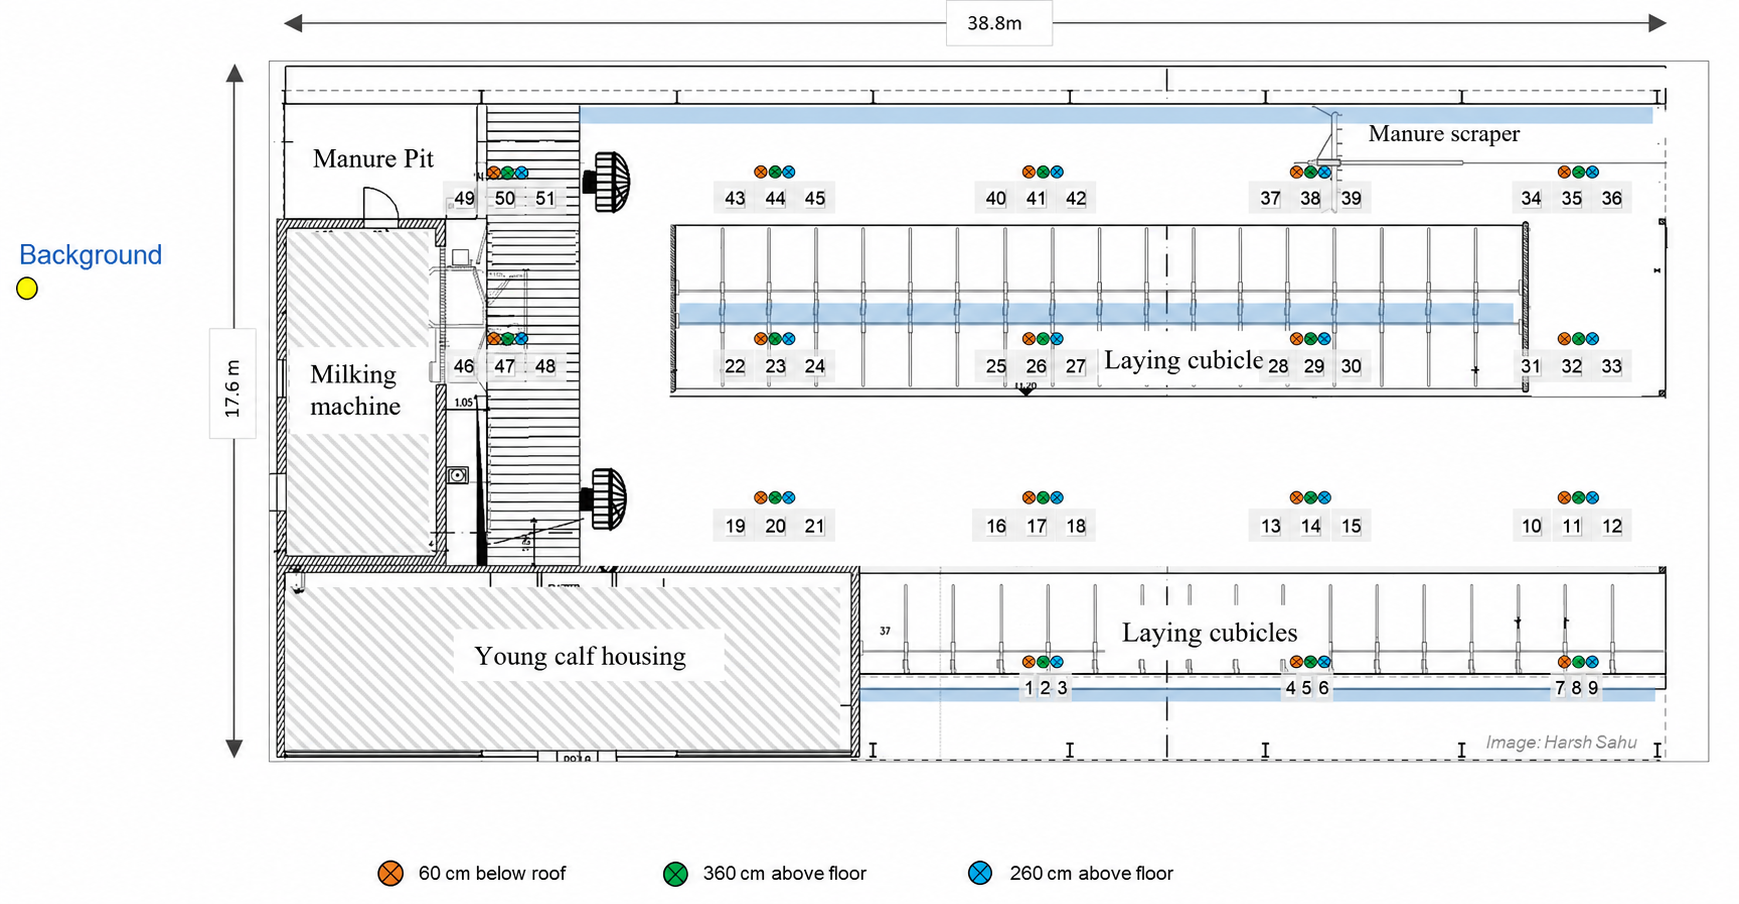
\includegraphics[width=\linewidth]{Fig1a_campaign1_sampling_layout_no_ringline.png}
\caption{Plan view and 51 internal SPs.}
\end{subfigure}
\begin{subfigure}[t]{0.83\textwidth}\centering
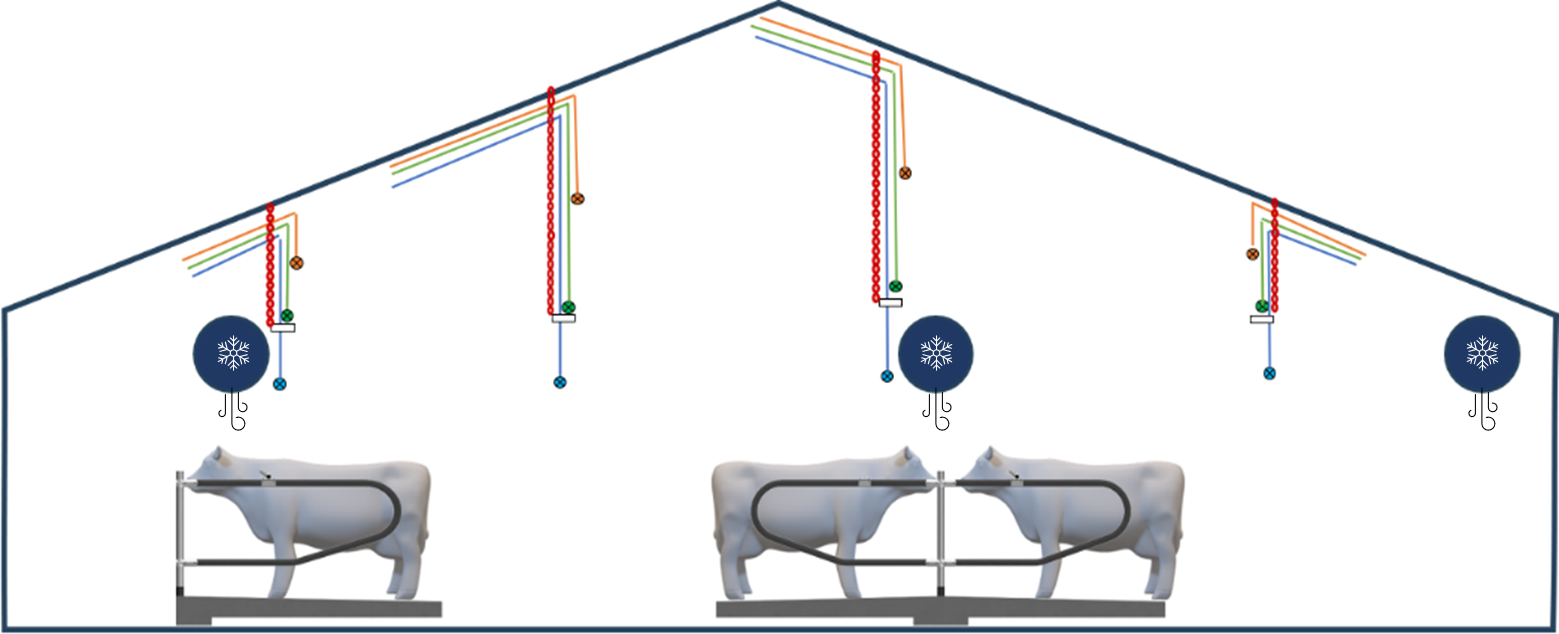
\includegraphics[width=\linewidth]{Fig1b_barn_cross_section.png}
\caption{Vertical arrangement of the sampling lines.}
\end{subfigure}
\caption{Experimental barn and dense Campaign~1 sampling design. Numbers are arranged in vertical triplets (top, middle and bottom). Functional zones and internal circulation fans are shown to support physical interpretation of the concentration field.}
\label{fig:layout}
\end{figure}

\subsection{Gas analysers and multiplexer allocation}

Gas concentrations were measured with two Fourier-transform infrared spectrometers (FTIR1 and FTIR2; Gasmet CX4000, Gasmet Technologies Oy, Finland) and two cavity ring-down spectrometers (CRDS8 and CRDS9; Picarro G2508 and G2509, Picarro Inc., USA). The analysers quantified \(\mathrm{CO_2}\), \(\mathrm{CH_4}\), \(\mathrm{NH_3}\) and water vapour. The CRDS instruments were each coupled to a 16-port multiposition valve; the FTIR instruments were connected to their respective multiplexed sampling channels. During Campaign~1, the 51 internal lines were divided among the four analysers: CRDS9 measured SP1--SP16, FTIR2 SP17--SP26, CRDS8 SP27--SP42 and FTIR1 SP43--SP51. The outside line was measured by FTIR1. An analyser-to-SP allocation table is provided in the Supplementary material so that spatial patterns can be audited for possible analyser assignment effects.

\subsection{Sampling sequence and temporal alignment}

The target residence time at each valve position was \SI{240}{s}. FTIR observations were exported as one value per sampling step. CRDS instruments recorded approximately one observation per second. For CRDS data, the first \SI{60}{s} following a valve change were discarded digitally to represent line flushing, and the remaining \SI{180}{s} were averaged. Each resulting record was stamped at the end of the sampling step. The cleaned analyser tables were then harmonised to the columns date--time, analyser, sampling port, SP, \(\mathrm{CO_2}\), \(\mathrm{CH_4}\), \(\mathrm{NH_3}\) and \(\mathrm{H_2O}\), and were appended row-wise.

Because four instruments sampled different parts of the network in parallel but each instrument switched sequentially among its assigned lines, the 51-point field was not observed instantaneously. A complete traversal of the analyser allocations lasted less than two hours. Two-hour blocks were therefore used when a contemporaneous whole-network summary was required. This blocking limits, but cannot eliminate, confounding between spatial differences and short-term changes in wind, animal activity or management.

\subsection{Campaigns}

Campaign~1 was the primary high-density experiment. Measurements covered summer 2024 and an autumn period from 1 to 24 October 2024. The two CRDS and two FTIR analysers were used to obtain the complete 51-SP configuration. Campaign~2 covered 16 November to 31 December 2024. Technical defects in the FTIR instruments prevented continuation of the four-analyser network. The sampling configuration was therefore adapted to the 32 available CRDS ports. Middle SPs were removed and the remaining top and bottom lines, including SP19 and SP40, were reassigned sequentially to CRDS8 and CRDS9. Sparse FTIR observations at SP49 and SP51 were preserved in the data archive but were not considered part of the inferential Campaign~2 network. Campaign~2 was thus a pragmatic seasonal extension, not an independent replication of the 51-SP experiment or a prior demonstration that the middle layer was redundant.

\subsection{Instrument comparability and quality assurance}

Before Campaign~1, all four analysers were operated for 24 h at a common position in the centre of the barn. Two PTFE lines terminated at the same suction location; one line was divided between the CRDS instruments and the other between the FTIR instruments. Relative to CRDS, the FTIR instruments reported concentrations approximately 6\% higher for \(\mathrm{CO_2}\) and \(\mathrm{CH_4}\), and 9\% higher for \(\mathrm{NH_3}\). Campaign~1 FTIR concentrations were therefore harmonised to the CRDS scale using 1.06 correction factors for \(\mathrm{CO_2}\), \(\mathrm{CH_4}\) and 1.09 \(\mathrm{NH_3}\). Before and after the field deployment, the analysers were additionally tested with nominal test-gas concentrations of \SI{700}{ppm} \(\mathrm{CO_2}\), \SI{7}{ppm} \(\mathrm{CH_4}\) and \SI{5}{ppm} \(\mathrm{NH_3}\). These test cylinder checks were treated as analyser accuracy checks.

\subsection{Meteorological context}

Hourly air temperature, relative humidity, precipitation, wind speed and wind direction were obtained from the German Meteorological Service for the nearest suitable station and aligned with the concentration records. These data described the seasonal and synoptic context of the two campaigns. They were not interpreted as direct measurements of velocity or flow direction at the barn openings. Consequently, meteorological comparisons were used to support interpretation of changing dispersion conditions, not to assign individual SP differences to a unique ventilation pathway.

\subsection{Analysis framework}

The analysis was organised around the single spatial-structure hypothesis. Concentrations and the dimensionless ratios \(\mathrm{CH_4}/\mathrm{CO_2}\), \(\mathrm{NH_3}/\mathrm{CO_2}\) and \(\mathrm{NH_3}/\mathrm{CH_4}\) were compared across height, horizontal position and time. Missing, zero and negative concentrations were excluded response-wise; no lower threshold was imposed on positive \(\mathrm{CO_2}\) observations. No observations were removed using a 1.5-interquartile-range rule or other statistical outlier filter. Arithmetic means and standard deviations described concentration magnitude and temporal dispersion, whereas medians and median absolute deviations provided robust summaries for the skewed distributions.

Clock-aligned two-hour blocks were used as the inferential unit. A sampling-point median was calculated within each block. Network-level analyses required at least 80\% of the maximum number of eligible SPs observed for the respective campaign and response. The reference for SP~\(i\) was the median of all other eligible SPs within the same block, thereby preventing the evaluated SP from contributing to its own reference. Signed relative error, absolute relative error, conventional coefficient of variation (CV), robust CV, and Spearman correlation with the leave-one-out reference were calculated for every SP. The robust CV was defined as \(100(1.4826\,\mathrm{MAD})/\mathrm{median}\). Paired Wilcoxon signed-rank tests evaluated whether blockwise SP-minus-reference differences were centred on zero; multiplicity was controlled within each campaign and response using the Holm procedure. Effect magnitude, rather than significance alone, was used to rank representative SPs.

Vertical effects were evaluated with mixed-effects models fitted to log-transformed two-hour medians. Height was a fixed effect, horizontal position an adjustment factor and two-hour block a random intercept. Campaign~1 models compared top, middle and bottom; Campaign~2 compared top and bottom. Estimated marginal means were back-transformed. Holm-adjusted height contrasts were expressed as ratios with 95\% confidence intervals. Temporal variability was also summarised at two-hour, daily, weekly and campaign scales. Spatial Shannon entropy was normalised by \(\ln(n)\) within each two-hour block. Temporal entropy was calculated for each SP using common bins within each campaign and response. Entropy was interpreted as information distribution, not as direct proof of airflow or physical mixing. Principal-component analysis and hierarchical pattern diagnostics were used as complementary exploratory analyses.

\subsection{Standard \texorpdfstring{\(\mathrm{CO_2}\)}{CO2}-balance ventilation and emission calculation}

The propagation of spatial concentration differences into ventilation and emission estimates was evaluated using a standard-input \(\mathrm{CO_2}\)-balance calculation. For every two-hour block, the median of the eligible internal SPs was paired with the contemporaneous outside line. Standard animal inputs were fixed at 58 dairy cows of \SI{500}{kg} liveweight, \SI{31.22}{kg\,cow^{-1}\,d^{-1}} milk production and a mean pregnancy day of 119.55. Heat production was calculated as
\begin{equation}
\Phi = 5.6m^{0.75}+22Y+1.6\times10^{-5}p^3,
\end{equation}
where \(m\) is liveweight (kg), \(Y\) is milk production (kg cow\(^{-1}\) d\(^{-1}\)) and \(p\) is pregnancy day. Carbon dioxide production was fixed at \SI{0.185}{m^3\,h^{-1}} per heat-production unit, giving \(P_{\mathrm{CO_2}}=\SI{14.016}{m^3\,h^{-1}}\) for the barn. The ventilation rate was
\begin{equation}
Q=\frac{P_{\mathrm{CO_2}}\,10^6}{C_{\mathrm{CO_2,in}}-C_{\mathrm{CO_2,out}}},
\end{equation}
and pollutant emission was
\begin{equation}
E_g=Q\left(C_{g,\mathrm{in}}-C_{g,\mathrm{out}}\right),
\end{equation}
after conversion of ppm to \si{mg\,m^{-3}} using DWD air temperature and an assumed pressure of \SI{101325}{Pa}. Rates were normalised to one \SI{500}{kg} livestock unit (LU). Annualised rate equivalents were calculated as \(E_g\times8760/1000\); these express persistence of the observed hourly rate and are not seasonally weighted annual inventories.

All calculation rows were retained for auditing. Primary summaries required a positive \(\mathrm{CO_2}\) enhancement of at least \SI{200}{ppm}; \SIrange{70}{199}{ppm} was retained for sensitivity analysis, and non-positive enhancements produced no ventilation estimate. Negative pollutant enhancements were retained in the unfiltered output because they diagnose background-reference mismatch, but were not interpreted as physical negative emissions. Campaign~2 contained only six network blocks with a contemporaneous outside reference and was therefore excluded from comparative emission inference.

\section{Results}

\subsection{Data coverage and temporal aggregation}

Campaign~1 provided valid positive observations from all four analysers at all 51 internal SPs. For each gas, approximately 30,181 CRDS9, 33,950 CRDS8, 39,861 FTIR1 and 40,018 FTIR2 observations were available after response-wise validity checks; the corresponding FTIR1 count for \(\mathrm{NH_3}\) was 39,277. The two-hour aggregation yielded 1,338 candidate blocks. Of these, 1,010 blocks met the 80\% spatial-coverage requirement for every concentration and ratio response, and the median valid block contained all 51 SPs.

Campaign~2 contributed 16,566 valid positive observations per gas from CRDS9 and 4,068 from CRDS8. The inferential network comprised 32 CRDS-connected top and bottom SPs, including SP19 and SP40. Of 552 candidate two-hour blocks, 136 met the 80\% coverage requirement. The median candidate block contained 16 SPs because the two CRDS sampling cycles were not always contemporaneously complete, whereas accepted blocks contained at least 26 of the 32 expected SPs. The sparse Campaign~2 FTIR2 records were retained in the archive but excluded from inference.

\begin{table}[htbp]
\centering
\caption{Measurement coverage and two-hour blocks used for network-level analyses. Valid positive observations are reported per gas; the \(\mathrm{NH_3}\) count for FTIR1 in Campaign~1 was 39,277. A valid network block contained at least 80\% of the maximum eligible SP count for the campaign.}
\label{tab:coverage}
\small
\resizebox{\textwidth}{!}{%
\begin{tabular}{llrrrr}
\toprule
Campaign & Analyser/network & Valid observations & Candidate blocks & Valid blocks & Eligible SPs\\
\midrule
1 & CRDS9 & 30,181 & -- & -- & 16\\
1 & CRDS8 & 33,950 & -- & -- & 16\\
1 & FTIR1 & 39,861 & -- & -- & 9\\
1 & FTIR2 & 40,018 & -- & -- & 10\\
1 & Complete network & -- & 1,338 & 1,010 & 51\\
2 & CRDS9 & 16,566 & -- & -- & 16\\
2 & CRDS8 & 4,068 & -- & -- & 16\\
2 & CRDS network & -- & 552 & 136 & 32\\
\bottomrule
\end{tabular}}
\end{table}

\subsection{Concentration distributions across sampling points}

The concentration distributions were right-skewed, with the extent of skewness differing among gases and ratios. Across SPs, the median absolute difference between the mean and median of the two-hour summaries was approximately 1.1\% for \(\mathrm{CO_2}\) in both campaigns. It was 1.7 and 3.6\% for \(\mathrm{CH_4}\), and 4.0 and 3.9\% for \(\mathrm{NH_3}\), in Campaigns~1 and 2, respectively. The largest mean--median separation occurred for \(\mathrm{NH_3}/\mathrm{CH_4}\), for which the corresponding median differences were 9.4 and 8.2\%. Nevertheless, mean- and median-based SP rankings were strongly associated (Spearman \(\rho=0.955\)--0.995 across responses and campaigns). Mean~\(\pm\)~SD was therefore retained for descriptive presentation, whereas median-based errors were used to evaluate typical representativeness.

\begin{figure}[htbp]
\centering
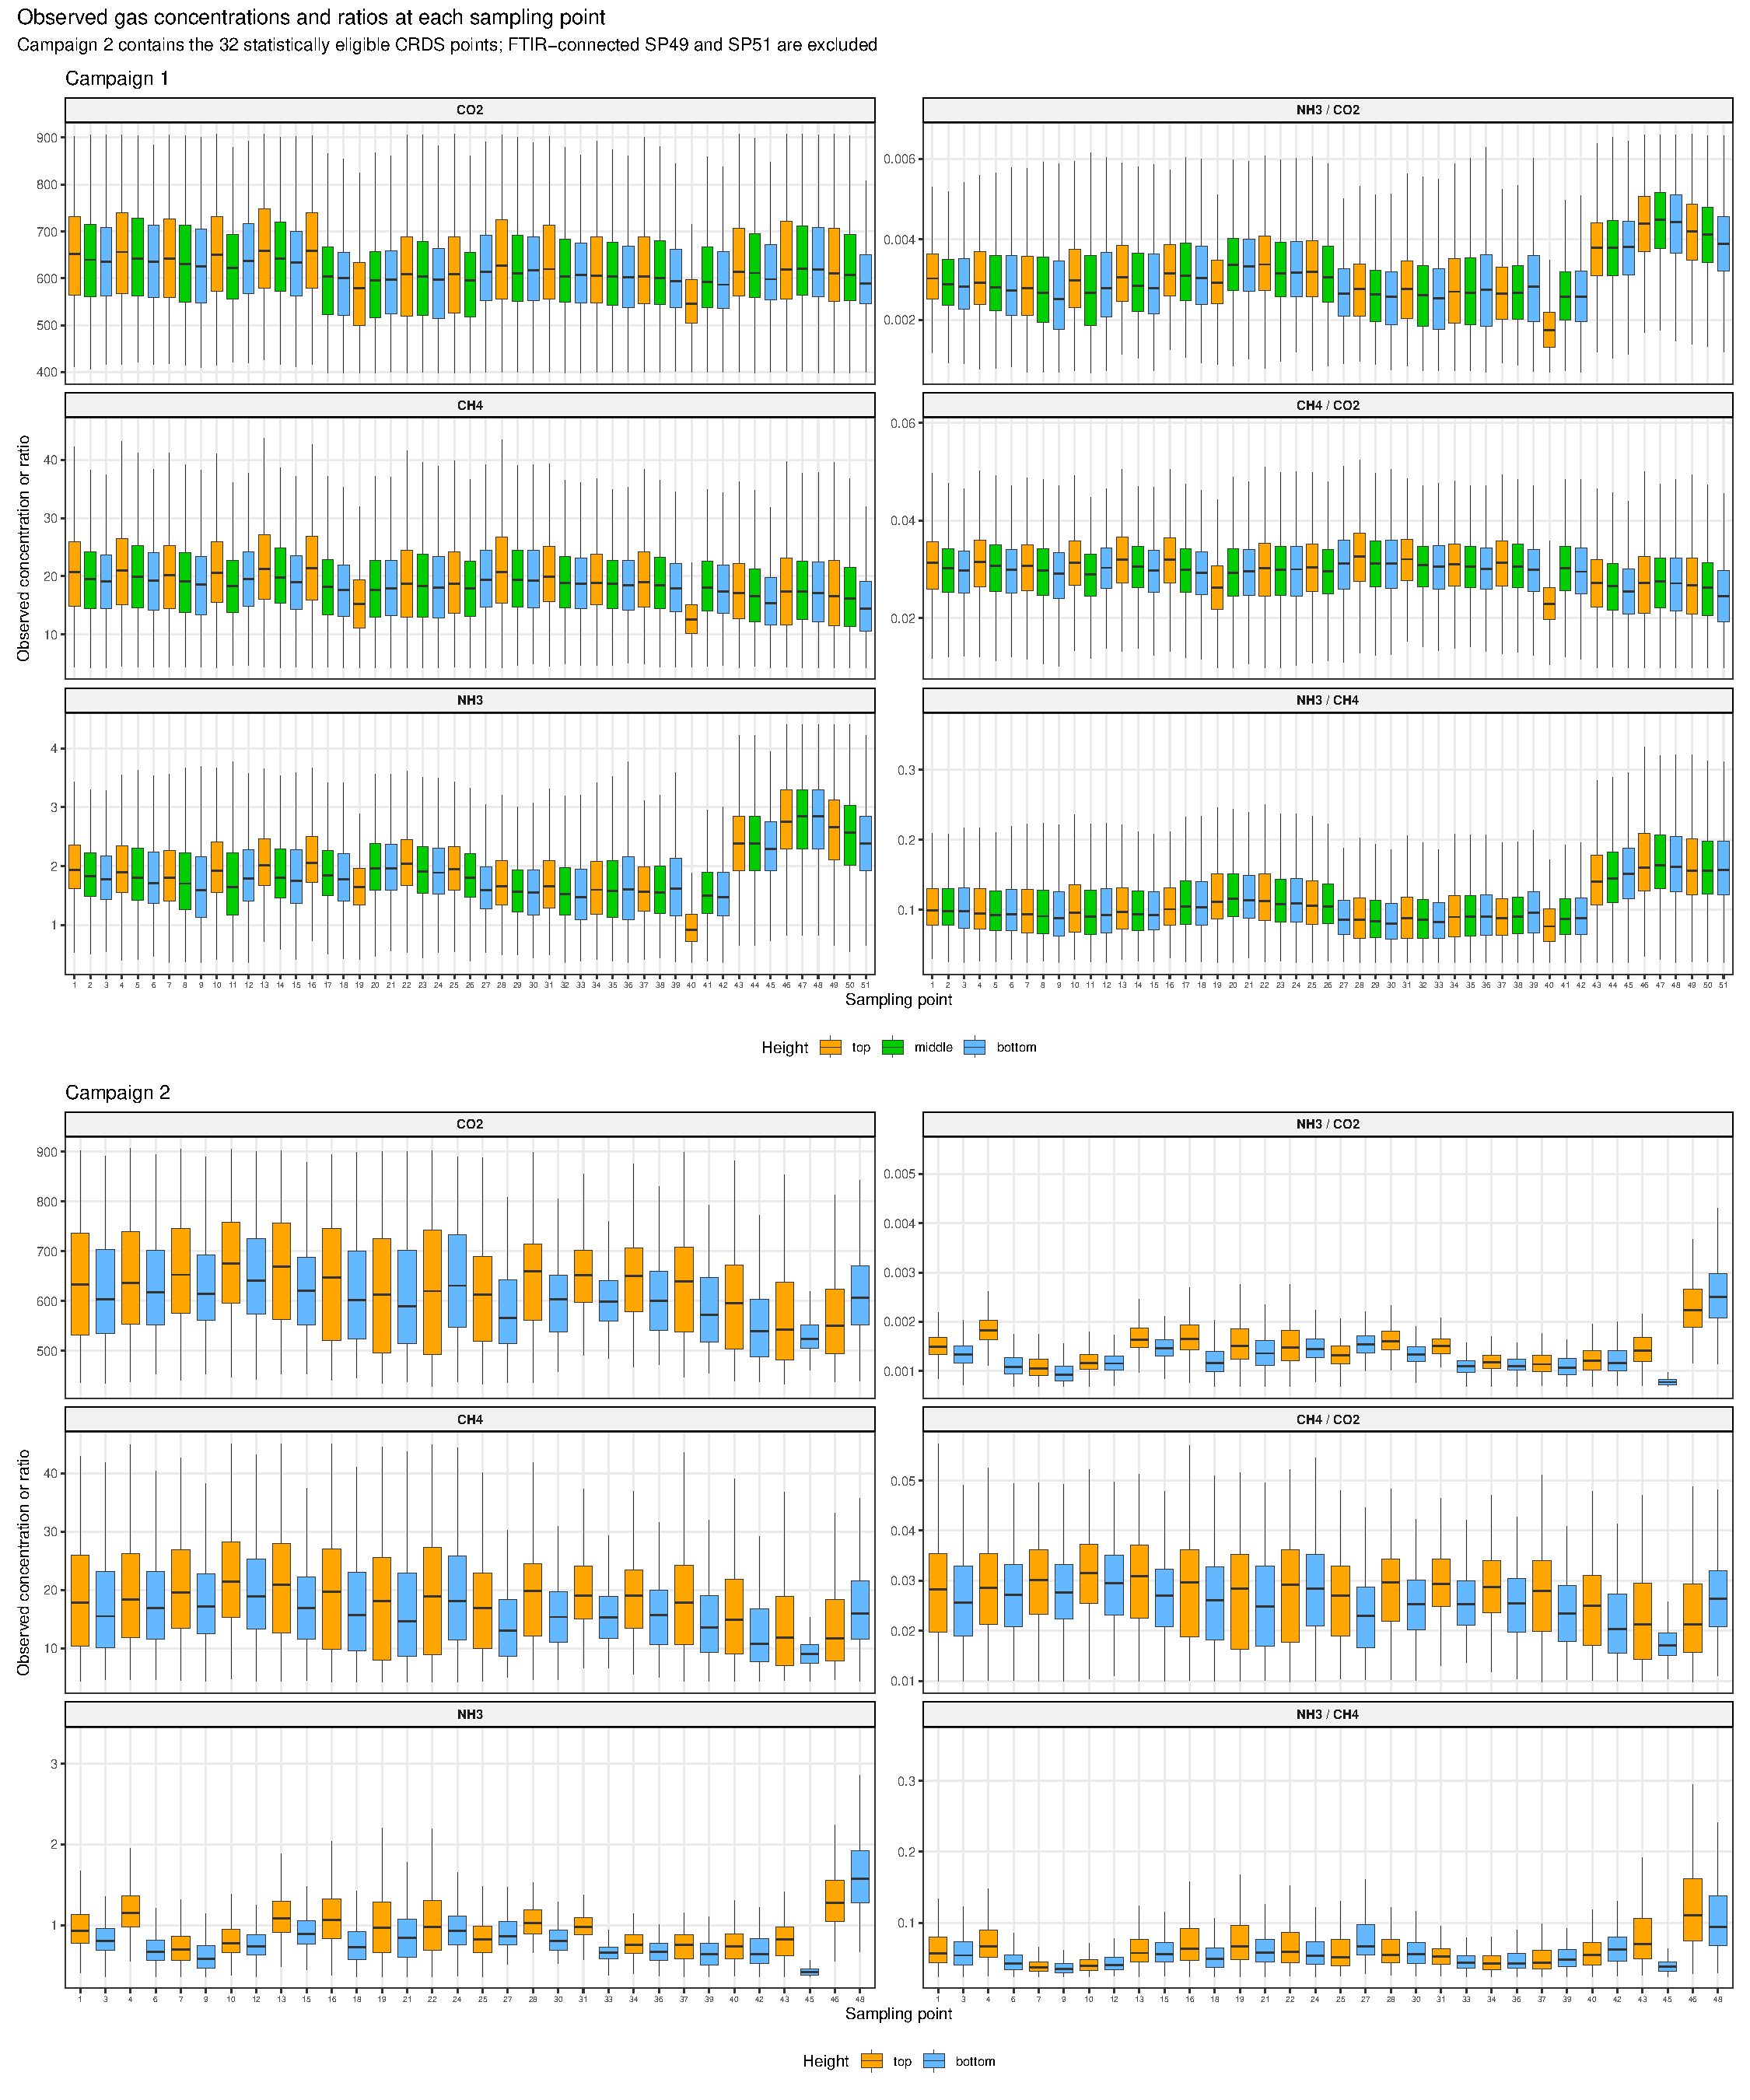
\includegraphics[width=\textwidth]{Fig_11_observed_SP_boxplots_campaign1_2_main.pdf}
\caption{Observed distributions of \(\mathrm{CO_2}\), \(\mathrm{CH_4}\), \(\mathrm{NH_3}\) and their dimensionless ratios at the eligible sampling points in Campaigns~1 and 2. Boxes show medians and interquartile ranges; extreme observations were retained in the analysis but omitted as individual boxplot symbols to preserve readability. Colours indicate vertical level: top, orange; middle, green; bottom, blue. Campaign~2 contains top and bottom SPs only.}
\label{fig:sp-boxplots}
\end{figure}

In Campaign~1, the mean two-hour concentrations at the top, middle and bottom levels were 628.8, 621.2 and 616.5~ppm for \(\mathrm{CO_2}\); 19.23, 18.78 and 18.44~ppm for \(\mathrm{CH_4}\); and 1.99, 1.97 and 1.92~ppm for \(\mathrm{NH_3}\), respectively. Campaign~2 top and bottom means were 643.8 and 620.3~ppm for \(\mathrm{CO_2}\), 18.97 and 17.08~ppm for \(\mathrm{CH_4}\), and 0.99 and 0.80~ppm for \(\mathrm{NH_3}\). The SDs were large relative to the means, especially for \(\mathrm{CH_4}\) and \(\mathrm{NH_3}\), demonstrating substantial temporal dispersion within every height group.

\begin{figure}[htbp]
\centering
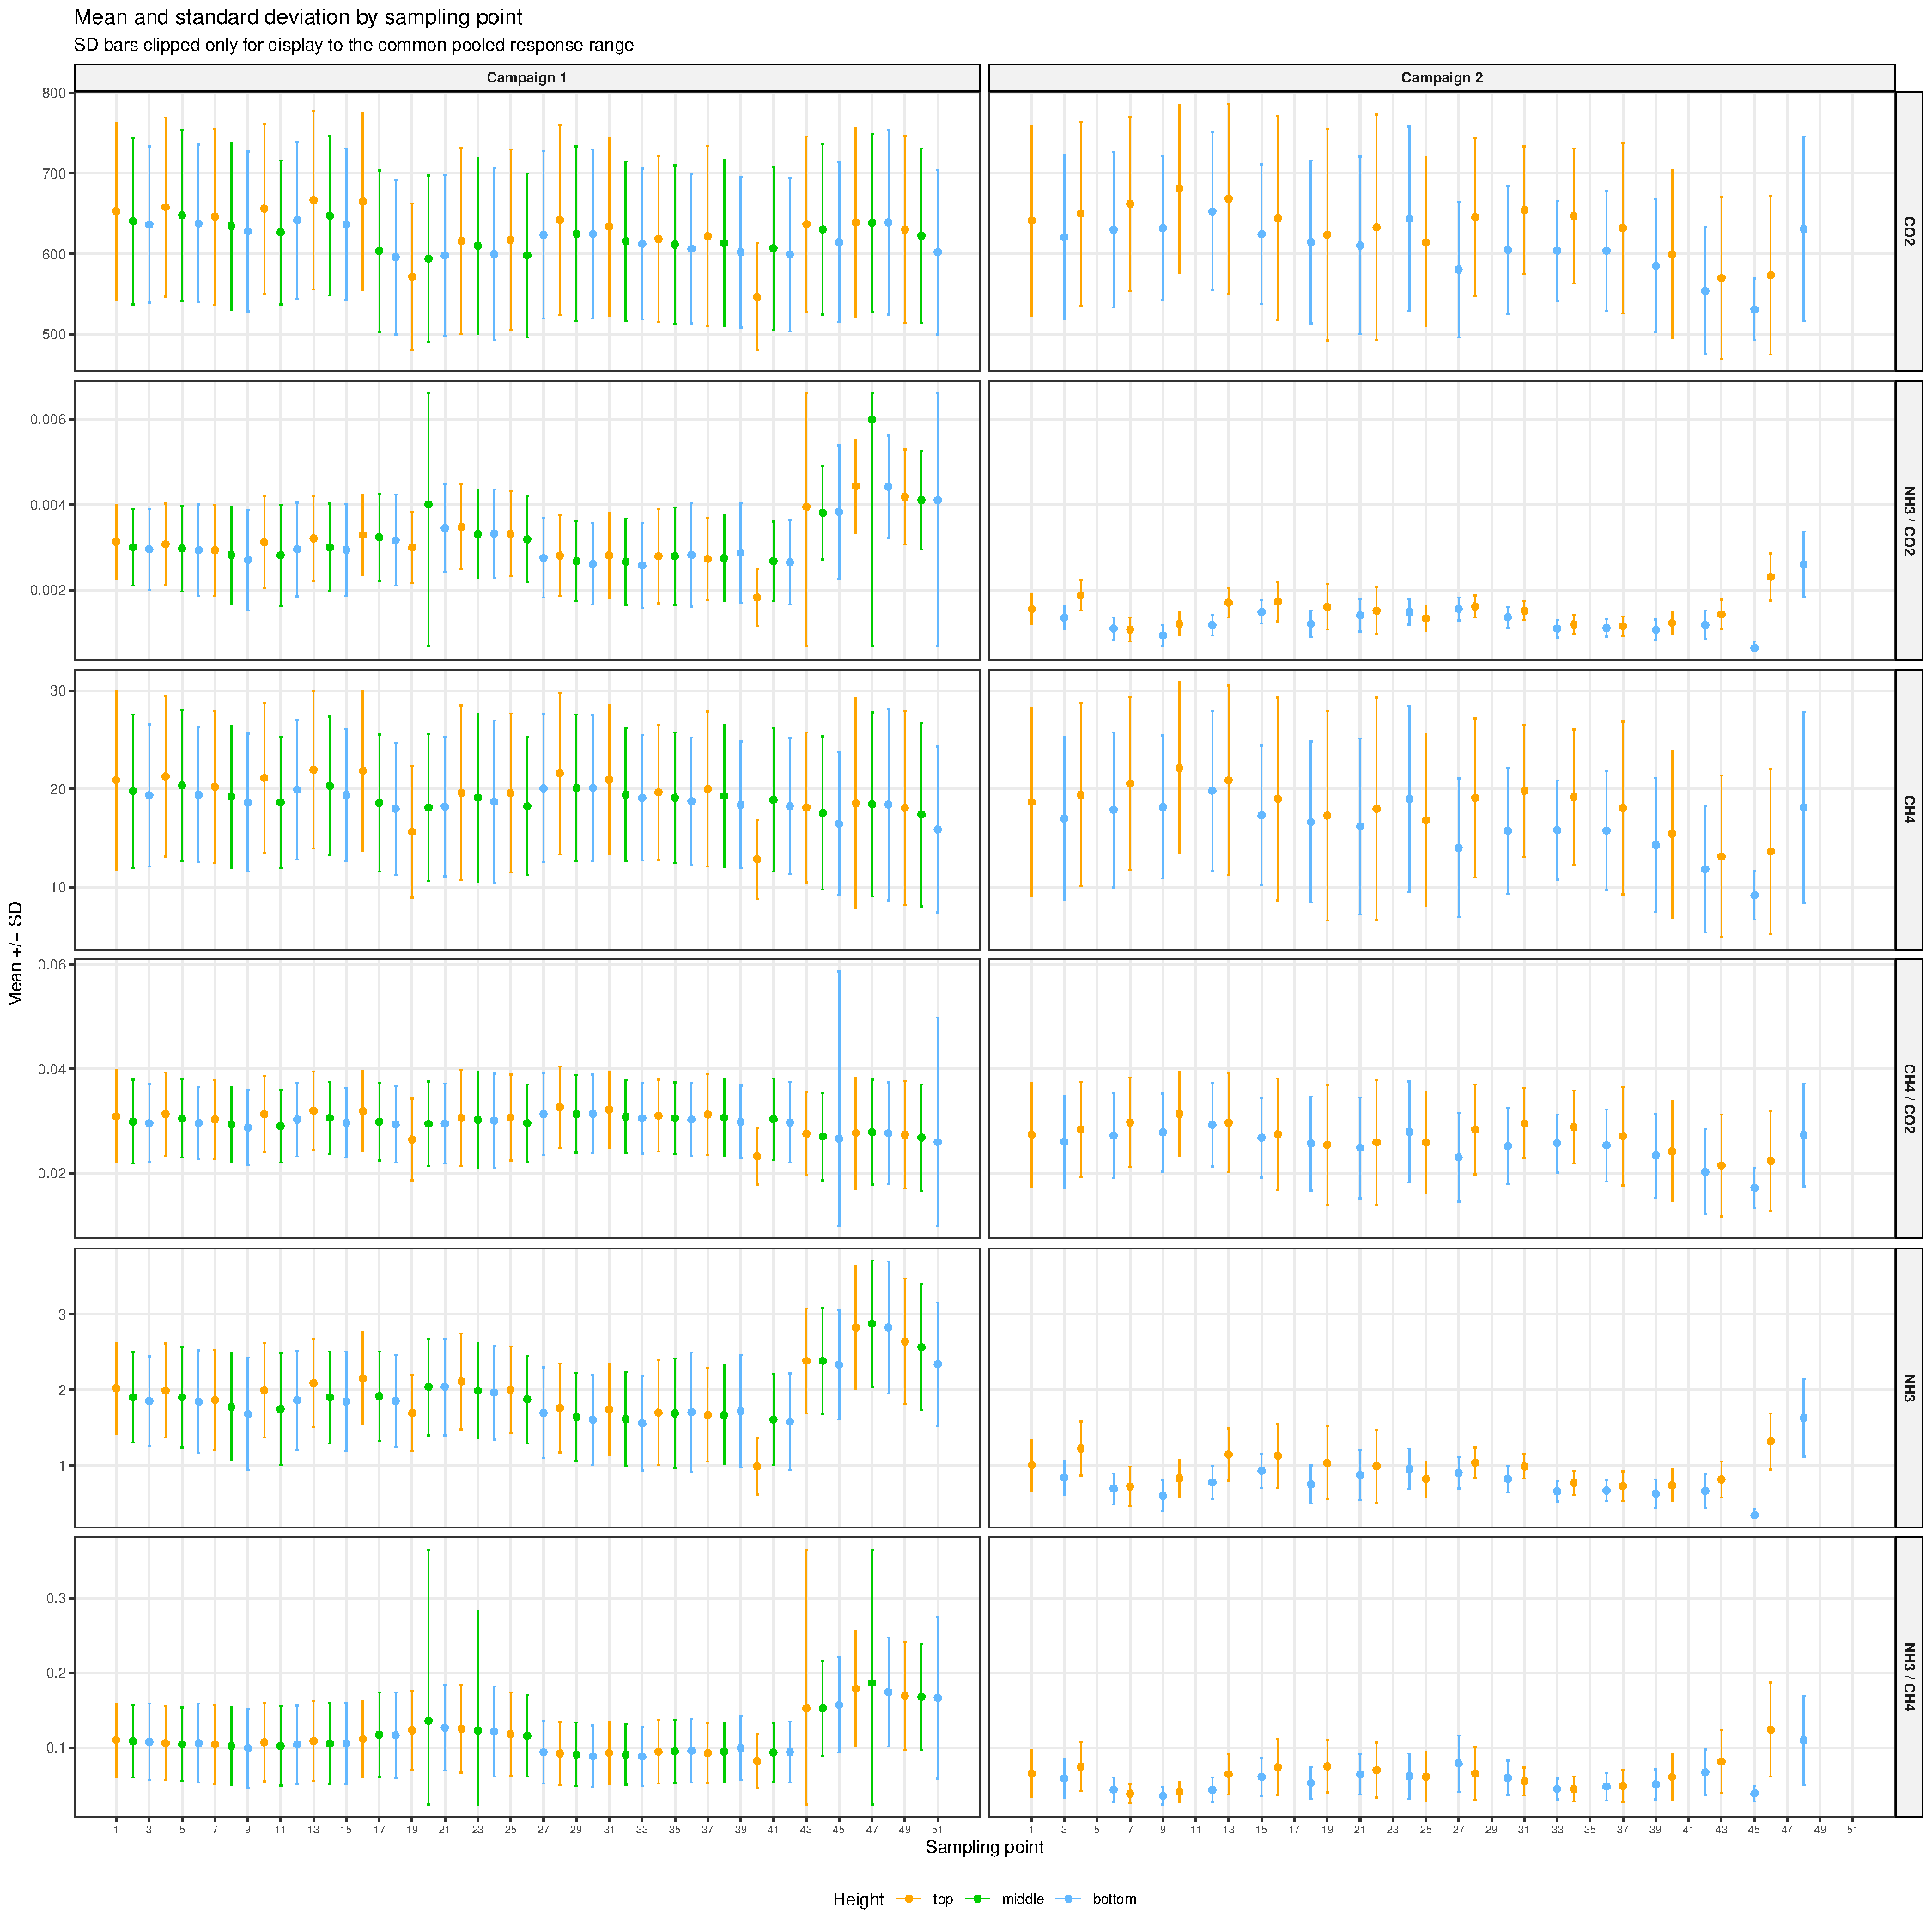
\includegraphics[width=\textwidth]{Fig_02_mean_plus_minus_SD_campaign1_2.pdf}
\caption{Arithmetic mean and standard deviation of gas concentrations and dimensionless gas ratios at each eligible SP. The full values were retained in the statistical tables; display limits were based on the pooled 0.5--99.5 percentile range for each response so that isolated extreme values did not obscure spatial patterns. Colours indicate top (orange), middle (green) and bottom (blue) sampling levels.}
\label{fig:mean-sd}
\end{figure}

\subsection{Vertical concentration structure}

All planned height contrasts were significant after multiplicity adjustment. In Campaign~1, the estimated top-to-bottom ratios were 1.017 (95\% CI 1.015--1.019) for \(\mathrm{CO_2}\), 1.031 (1.026--1.036) for \(\mathrm{CH_4}\), and 1.045 (1.039--1.051) for \(\mathrm{NH_3}\). The top level was also higher than the middle level, with ratios of 1.010, 1.013 and 1.013, respectively. Middle-to-bottom ratios were 1.007 for \(\mathrm{CO_2}\), 1.017 for \(\mathrm{CH_4}\), and 1.032 for \(\mathrm{NH_3}\). Thus, the estimated ordering was top~\(>\)~middle~\(>\)~bottom for all three gases, although the proportional separation was gas-specific.

The top--bottom contrasts were larger in Campaign~2. Estimated ratios were 1.033 (95\% CI 1.031--1.036) for \(\mathrm{CO_2}\), 1.074 (1.064--1.084) for \(\mathrm{CH_4}\), and 1.228 (1.219--1.237) for \(\mathrm{NH_3}\). The largest vertical separation was therefore consistently observed for \(\mathrm{NH_3}\), followed by \(\mathrm{CH_4}\) and \(\mathrm{CO_2}\).

\begin{table}[htbp]
\centering
\caption{Mixed-effects model contrasts between vertical sampling levels. Ratios greater than one indicate a greater concentration at the first-named height. All contrasts were Holm-adjusted and significant at \(p<0.001\).}
\label{tab:height-contrasts}
\small
\begin{tabular}{llrrrr}
\toprule
Campaign & Response & Contrast & Ratio & 95\% CI lower & 95\% CI upper\\
\midrule
1 & \(\mathrm{CO_2}\) & Top/middle & 1.010 & 1.008 & 1.012\\
1 & \(\mathrm{CO_2}\) & Top/bottom & 1.017 & 1.015 & 1.019\\
1 & \(\mathrm{CO_2}\) & Middle/bottom & 1.007 & 1.005 & 1.009\\
1 & \(\mathrm{CH_4}\) & Top/middle & 1.013 & 1.008 & 1.018\\
1 & \(\mathrm{CH_4}\) & Top/bottom & 1.031 & 1.026 & 1.036\\
1 & \(\mathrm{CH_4}\) & Middle/bottom & 1.017 & 1.012 & 1.022\\
1 & \(\mathrm{NH_3}\) & Top/middle & 1.013 & 1.007 & 1.018\\
1 & \(\mathrm{NH_3}\) & Top/bottom & 1.045 & 1.039 & 1.051\\
1 & \(\mathrm{NH_3}\) & Middle/bottom & 1.032 & 1.026 & 1.038\\
2 & \(\mathrm{CO_2}\) & Top/bottom & 1.033 & 1.031 & 1.036\\
2 & \(\mathrm{CH_4}\) & Top/bottom & 1.074 & 1.064 & 1.084\\
2 & \(\mathrm{NH_3}\) & Top/bottom & 1.228 & 1.219 & 1.237\\
\bottomrule
\end{tabular}
\end{table}

\begin{figure}[htbp]
\centering
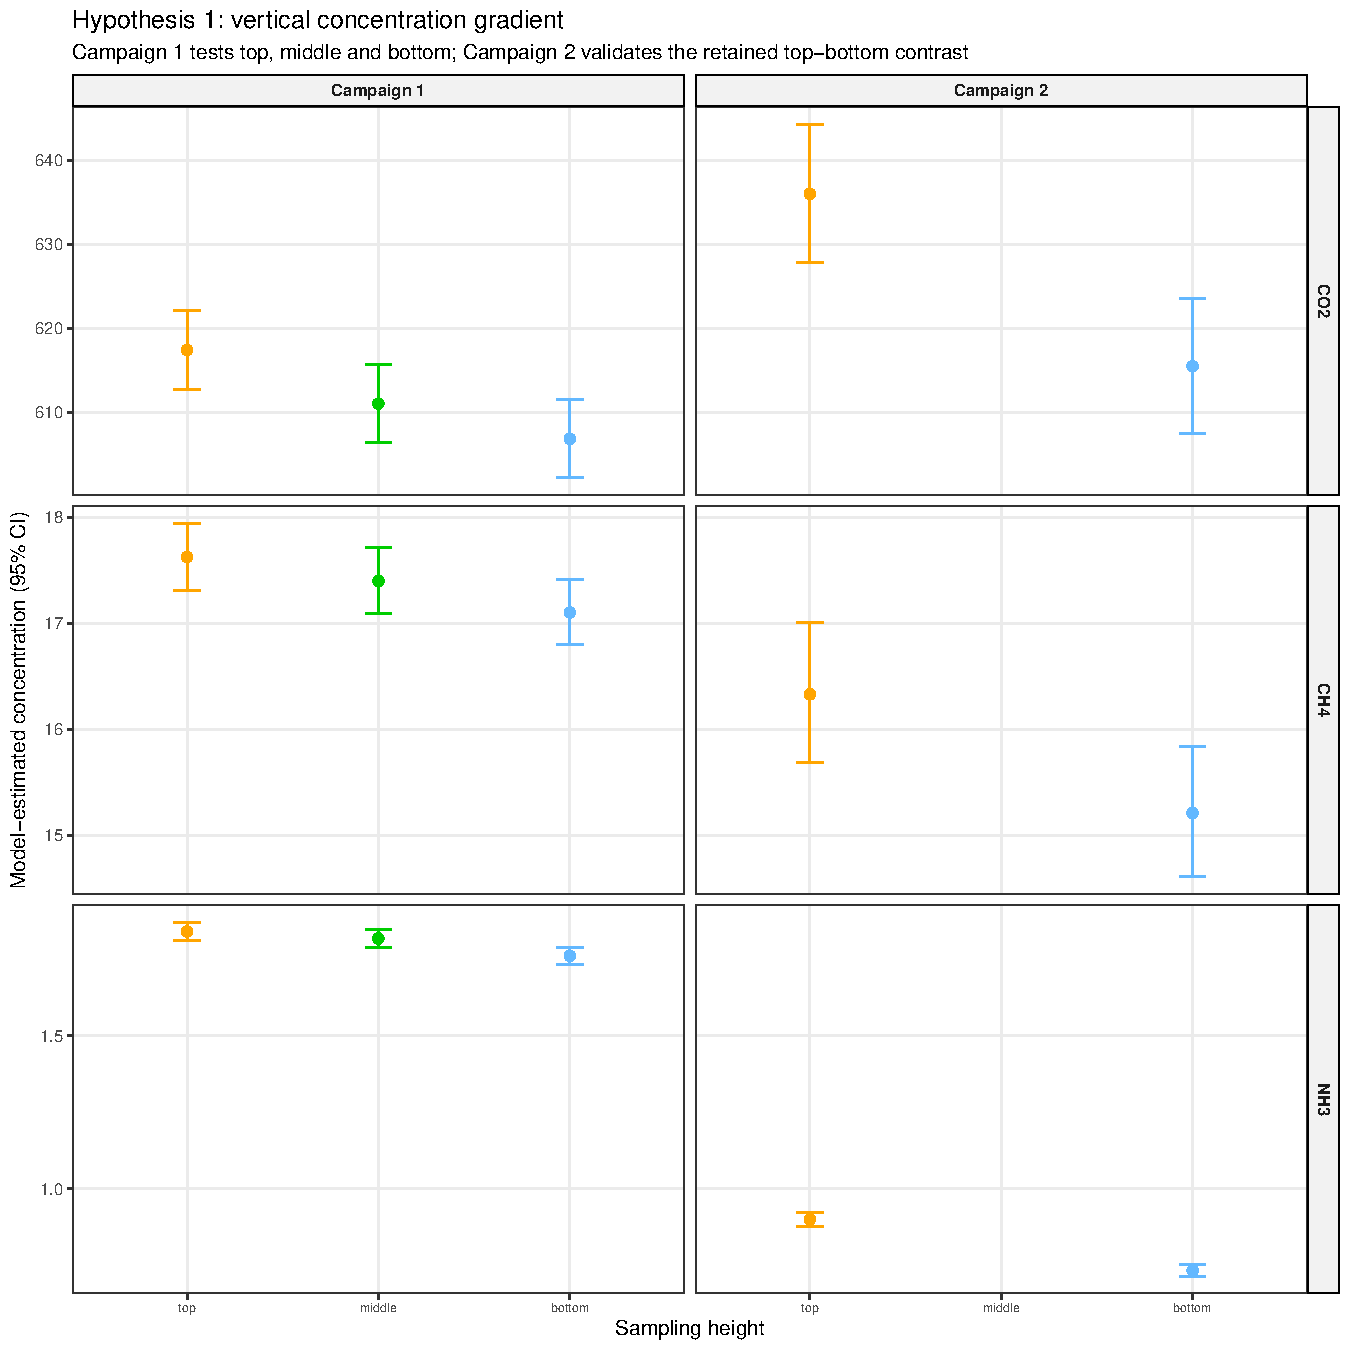
\includegraphics[width=0.88\textwidth]{Fig_06_H1_mixed_model_vertical_gradient.pdf}
\caption{Back-transformed estimated marginal means from the mixed-effects models of log-transformed two-hour concentration medians. Models included height as a fixed effect, horizontal position as an adjustment factor and two-hour block as a random intercept. Error bars are 95\% confidence intervals. Campaign~1 contains top, middle and bottom levels; Campaign~2 contains top and bottom levels.}
\label{fig:height-model}
\end{figure}

\subsection{Temporal variability and aggregation scale}

Spatial variability decreased as observations were aggregated over longer periods, but the extent of attenuation differed by gas. In Campaign~1, the median robust CV across SPs decreased from 7.6\% at the two-hour scale to 3.3\% at the campaign scale for \(\mathrm{CO_2}\), from 17.3 to 6.5\% for \(\mathrm{CH_4}\), and from 23.3 to 15.6\% for \(\mathrm{NH_3}\). In Campaign~2, the corresponding reductions were from 7.1 to 5.5\%, from 22.5 to 16.6\%, and from 24.4 to 23.0\%, respectively. The median spatial range also remained gas-specific. At the two-hour scale it was approximately 31.2, 78.3 and 105.6\% for \(\mathrm{CO_2}\), \(\mathrm{CH_4}\) and \(\mathrm{NH_3}\) in Campaign~1, and 25.1, 82.2 and 93.5\% in Campaign~2.

Conventional and robust CVs were broadly similar for many SPs but diverged at locations affected by episodic peaks or small ratio denominators. Consequently, CV alone did not identify whether a location was representative of the network: some low-CV SPs retained systematic signed errors, while some more variable SPs closely followed the contemporaneous network series.

\begin{figure}[htbp]
\centering
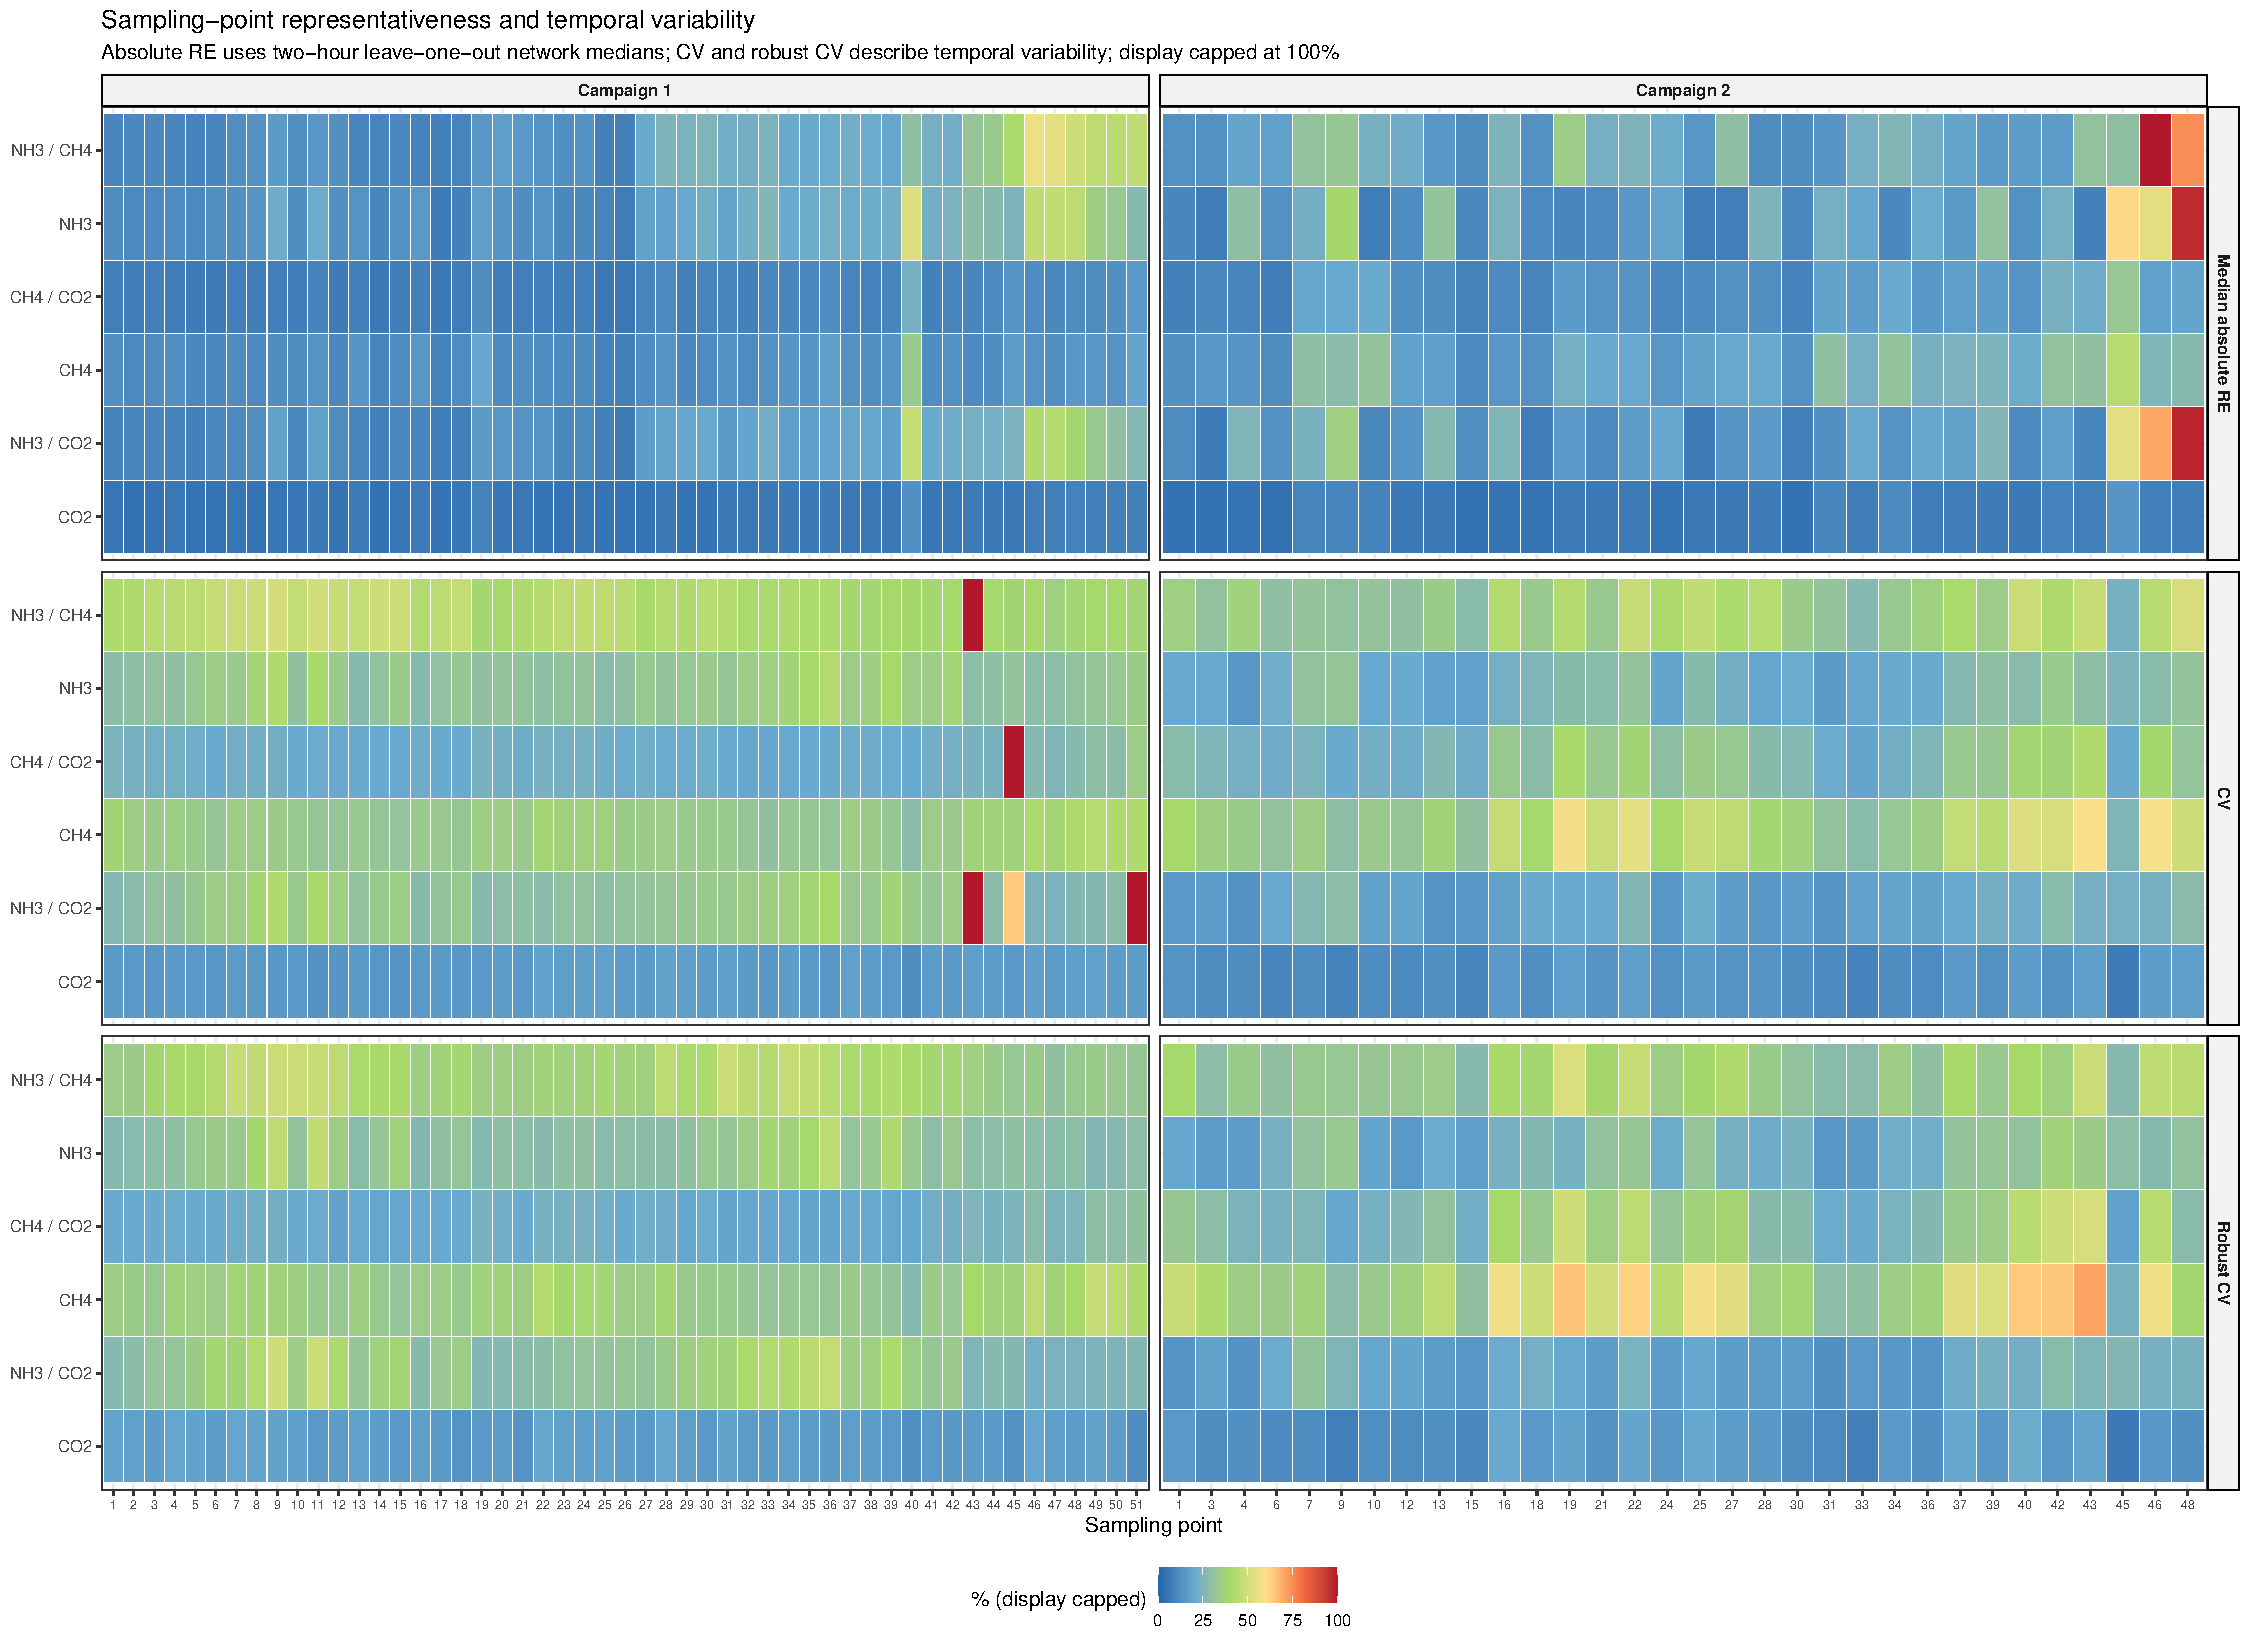
\includegraphics[width=\textwidth]{Fig_18_absolute_RE_CV_robustCV_heatmaps_campaign1_2.pdf}
\caption{Sampling-point representativeness and temporal variability. Median absolute relative error (RE) was calculated against the contemporaneous two-hour leave-one-out network median. Conventional CV was calculated as \(100\,\mathrm{SD}/\mathrm{mean}\), and robust CV as \(100(1.4826\,\mathrm{MAD})/\mathrm{median}\). Colour values are capped at 100\% for display; uncapped numerical values were retained in the statistical output.}
\label{fig:re-cv}
\end{figure}

\subsection{Sampling-point representativeness}

The SP with the smallest median absolute leave-one-out error depended on the response. In Campaign~1, the three closest SPs were SP14, SP2 and SP25 for \(\mathrm{CO_2}\); SP26, SP25 and SP17 for \(\mathrm{CH_4}\); and SP17, SP26 and SP18 for \(\mathrm{NH_3}\). For the ratios, SP26, SP25 and SP17 ranked highest for \(\mathrm{CH_4}/\mathrm{CO_2}\); SP26, SP17 and SP18 for \(\mathrm{NH_3}/\mathrm{CO_2}\); and SP25, SP26 and SP17 for \(\mathrm{NH_3}/\mathrm{CH_4}\). SP25 was therefore among the three closest locations for four of the six responses but was not universally optimal.

Median absolute relative errors for the best Campaign~1 SPs were approximately 4.1\% for \(\mathrm{CO_2}\), 8.0\% for \(\mathrm{CH_4}\), 6.7\% for \(\mathrm{NH_3}\), 5.3\% for \(\mathrm{CH_4}/\mathrm{CO_2}\), 6.4\% for \(\mathrm{NH_3}/\mathrm{CO_2}\), and 8.1\% for \(\mathrm{NH_3}/\mathrm{CH_4}\). In Campaign~2, minimum median absolute errors were 3.4\% for \(\mathrm{CO_2}\), 11.0\% for \(\mathrm{CH_4}\), 6.9\% for \(\mathrm{NH_3}\), 7.4\% for \(\mathrm{CH_4}/\mathrm{CO_2}\), 6.4\% for \(\mathrm{NH_3}/\mathrm{CO_2}\), and 11.9\% for \(\mathrm{NH_3}/\mathrm{CH_4}\). The identity of the highest-ranking Campaign~2 SP also varied by response.

After Holm adjustment, 48 of 51 Campaign~1 SPs differed from the leave-one-out reference for \(\mathrm{CO_2}\), 42 for \(\mathrm{CH_4}\), 46 for \(\mathrm{NH_3}\), 39 for \(\mathrm{CH_4}/\mathrm{CO_2}\), 50 for \(\mathrm{NH_3}/\mathrm{CO_2}\), and 47 for \(\mathrm{NH_3}/\mathrm{CH_4}\). Campaign~2 counts were 20, 21, 31, 22, 31 and 27 of 32 SPs, respectively. Given the large number of repeated blocks, these tests had high power; the magnitude and direction of the leave-one-out errors provided the principal ranking information.

\begin{table}[htbp]
\centering
\caption{Three SPs with the smallest median absolute relative error against the contemporaneous leave-one-out network median. Values in parentheses are median absolute errors (\%).}
\label{tab:representative-sp}
\small
\resizebox{\textwidth}{!}{%
\begin{tabular}{lll}
\toprule
Response & Campaign 1 & Campaign 2\\
\midrule
\(\mathrm{CO_2}\) & SP14 (4.10), SP2 (4.14), SP25 (4.24) & SP15 (3.40), SP6 (3.42), SP30 (3.82)\\
\(\mathrm{CH_4}\) & SP26 (7.98), SP25 (8.57), SP17 (9.02) & SP15 (11.03), SP6 (11.47), SP1 (12.61)\\
\(\mathrm{NH_3}\) & SP17 (6.74), SP26 (7.03), SP18 (8.29) & SP25 (6.95), SP3 (7.05), SP10 (7.17)\\
\(\mathrm{CH_4/CO_2}\) & SP26 (5.29), SP25 (5.63), SP17 (5.81) & SP6 (7.37), SP1 (8.26), SP15 (8.76)\\
\(\mathrm{NH_3/CO_2}\) & SP26 (6.36), SP17 (7.04), SP18 (7.57) & SP25 (6.39), SP3 (6.74), SP18 (7.01)\\
\(\mathrm{NH_3/CH_4}\) & SP25 (8.09), SP26 (8.16), SP17 (8.20) & SP30 (11.91), SP28 (11.91), SP15 (11.98)\\
\bottomrule
\end{tabular}}
\end{table}

\subsection{Spatial and temporal entropy}

Normalised spatial entropy was close to one for all responses, but small systematic differences were resolved. Median values in Campaign~1 were 0.999 for \(\mathrm{CO_2}\), 0.996 for \(\mathrm{CH_4}\), 0.991 for \(\mathrm{NH_3}\), 0.998 for \(\mathrm{CH_4}/\mathrm{CO_2}\), 0.993 for \(\mathrm{NH_3}/\mathrm{CO_2}\), and 0.990 for \(\mathrm{NH_3}/\mathrm{CH_4}\). Campaign~2 values were 0.999, 0.989, 0.988, 0.994, 0.989 and 0.984, respectively. The associated median information deficit was smallest for \(\mathrm{CO_2}\) and largest for \(\mathrm{NH_3}/\mathrm{CH_4}\) in both campaigns.

Temporal entropy varied more strongly among individual SPs than spatial entropy varied among complete blocks. Low temporal-entropy values were concentrated at a small number of SPs, but their identity was response- and campaign-specific. For example, SP40 had the lowest Campaign~1 temporal entropy for each concentration, whereas different Campaign~2 SPs occupied the lowest ranks. Entropy rankings therefore did not reproduce a single universal representative location and were retained as a complementary description of state occupancy rather than as the sole stability criterion.

\begin{figure}[htbp]
\centering
\begin{subfigure}[t]{0.98\textwidth}
\centering
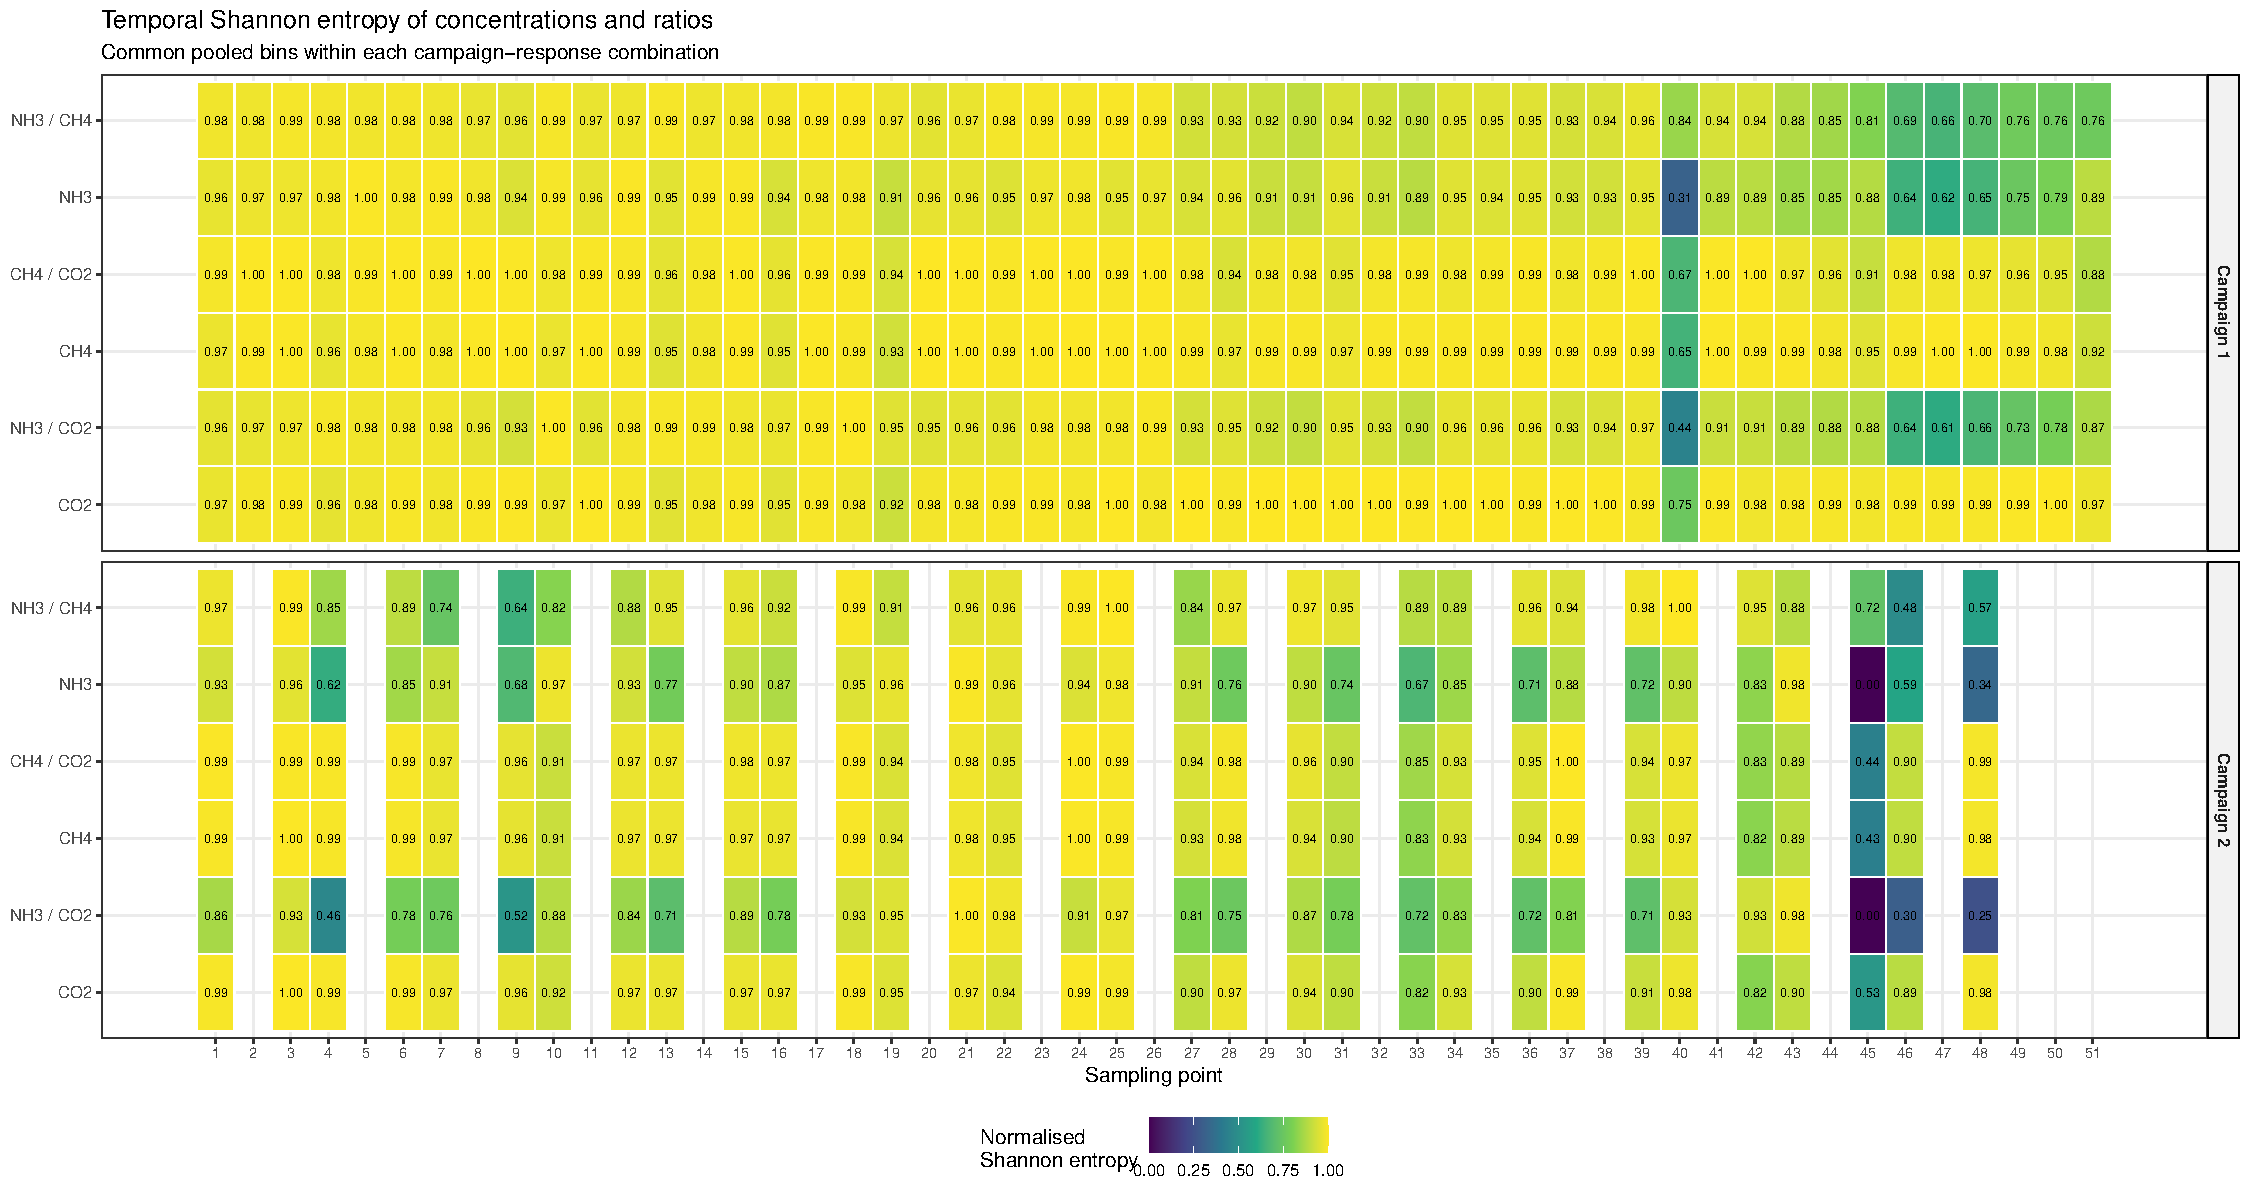
\includegraphics[width=\linewidth]{Fig_05_temporal_Shannon_entropy_campaign1_2.pdf}
\caption{Normalised temporal entropy by SP.}
\end{subfigure}
\vspace{0.5em}
\begin{subfigure}[t]{0.82\textwidth}
\centering
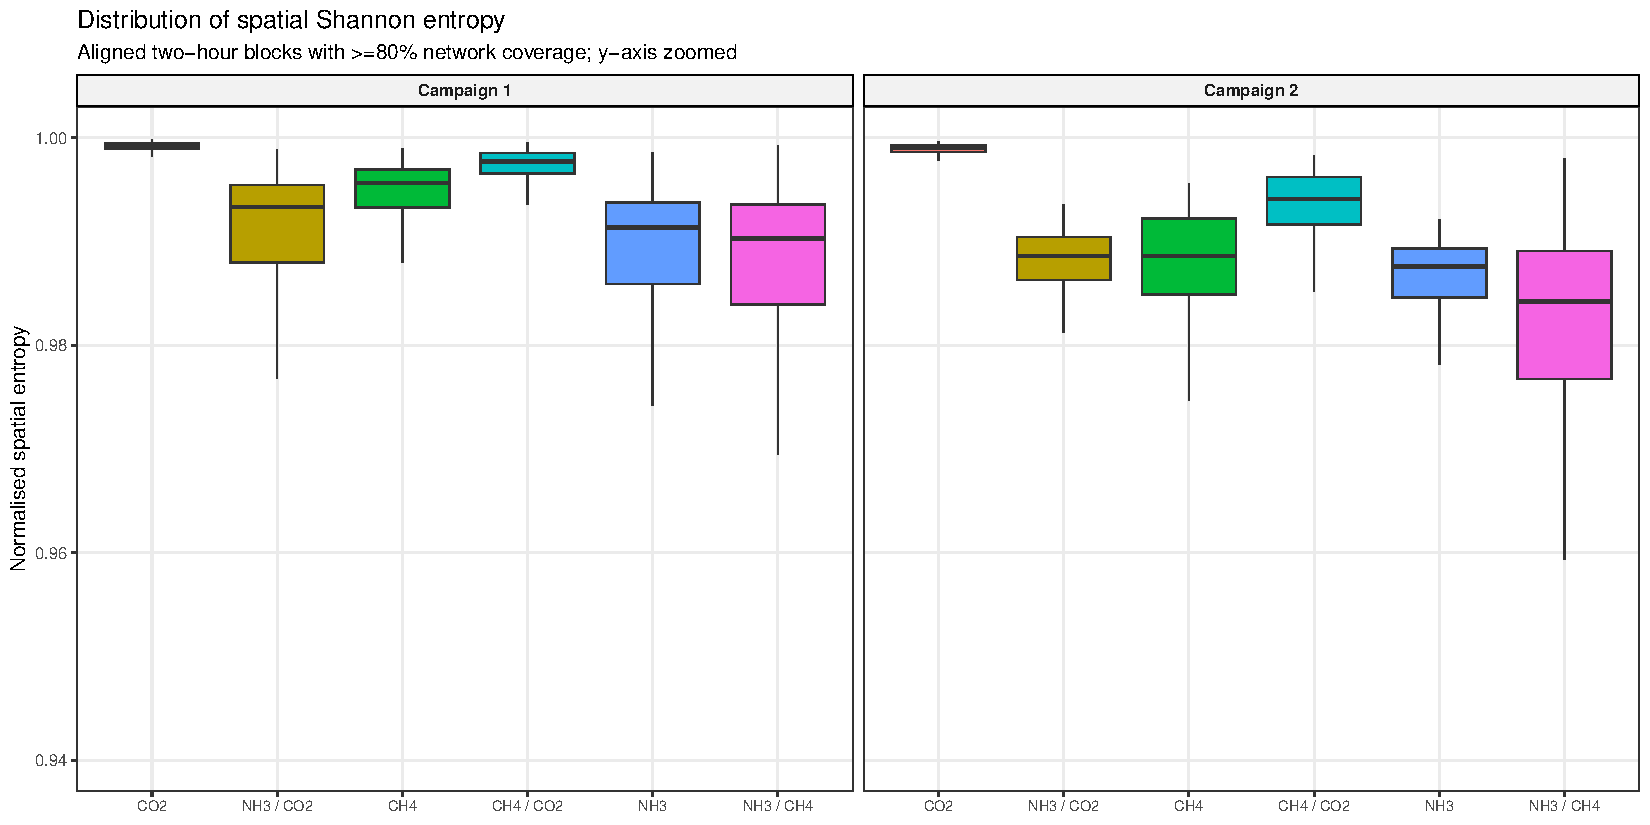
\includegraphics[width=\linewidth]{Fig_10_spatial_Shannon_entropy_distribution_campaign1_2.pdf}
\caption{Distribution of normalised spatial entropy across valid two-hour blocks.}
\end{subfigure}
\caption{Shannon entropy diagnostics for concentrations and dimensionless gas ratios. Temporal entropy used common bins within each campaign and response. Spatial entropy quantified the evenness of the concentration distribution over the eligible network and was normalised by \(\ln(n)\). Entropy was interpreted as information distribution rather than direct evidence of physical mixing.}
\label{fig:entropy}
\end{figure}

\subsection{Ventilation rate and emission estimates}

In Campaign~1, 473 network-median blocks met the primary \(\Delta\mathrm{CO_2}\geq\SI{200}{ppm}\) criterion for ventilation. The median ventilation rate was \SI{960.5}{m^3\,h^{-1}\,LU^{-1}} (interquartile range 796.9--1099.4), while the arithmetic mean was \SI{943.9}{m^3\,h^{-1}\,LU^{-1}}. Pollutant enhancements and emissions were finite in 464 of these blocks. Median \(\mathrm{CH_4}\) emission was \SI{12.73}{g\,h^{-1}\,LU^{-1}} (11.25--14.12), equivalent to \SI{111.5}{kg\,year^{-1}\,LU^{-1}} if the observed rate persisted throughout a year. Median \(\mathrm{NH_3}\) emission was \SI{0.969}{g\,h^{-1}\,LU^{-1}} (0.729--1.272), corresponding to an annualised rate equivalent of \SI{8.49}{kg\,year^{-1}\,LU^{-1}} (Table~\ref{tab:emissions}).

Sampling configuration affected \(Q\) more strongly than the median pollutant emissions because \(Q\) is inversely proportional to the selected \(\mathrm{CO_2}\) enhancement. Relative to the full 51-SP median, the top-only, middle-only and bottom-only configurations had median absolute ventilation errors of 6.50, 1.74 and 5.14\%, respectively. Retaining the 34 top-and-bottom SPs reduced the median absolute errors to 1.16\% for \(Q\), 1.44\% for \(\mathrm{CH_4}\) and 2.05\% for \(\mathrm{NH_3}\). The Campaign~2-like 32-SP configuration gave corresponding median errors of 1.74, 1.55 and 2.83\%. However, the 95th-percentile error was 7.59\% for \(Q\), 6.31\% for \(\mathrm{CH_4}\) and 16.06\% for \(\mathrm{NH_3}\), showing that agreement in the median did not remove episodic configuration sensitivity.

\begin{table}[htbp]
\centering
\caption{Standard-input \(\mathrm{CO_2}\)-balance ventilation and emission estimates for Campaign~1. Values are medians with interquartile ranges. Annual values are rate equivalents obtained by multiplying the hourly rate by 8760 h and are not seasonally weighted annual inventories.}
\label{tab:emissions}
\small
\begin{tabular}{lrrr}
\toprule
Metric & Valid blocks & Median & Interquartile range\\
\midrule
Ventilation (\si{m^3\,h^{-1}\,LU^{-1}}) & 473 & 960.49 & 796.91--1099.40\\
\(\mathrm{CH_4}\) (\si{g\,h^{-1}\,LU^{-1}}) & 464 & 12.73 & 11.25--14.12\\
\(\mathrm{CH_4}\) (\si{kg\,year^{-1}\,LU^{-1}}) & 464 & 111.52 & 98.52--123.69\\
\(\mathrm{NH_3}\) (\si{g\,h^{-1}\,LU^{-1}}) & 464 & 0.969 & 0.729--1.272\\
\(\mathrm{NH_3}\) (\si{kg\,year^{-1}\,LU^{-1}}) & 464 & 8.49 & 6.38--11.14\\
\bottomrule
\end{tabular}
\end{table}

\section{Discussion}

\subsection{A structured, gas-specific concentration field}

The dense network rejected the simplifying assumption that the upper barn airspace was spatially homogeneous. The consistent top--middle--bottom ordering in Campaign~1, and the larger top--bottom contrasts in Campaign~2, show that the vertical structure was reproducible after the instruments, season and sampling allocation changed. At the same time, the effect was gas-specific: the Campaign~1 top-to-bottom difference was only 1.7\% for \(\mathrm{CO_2}\), but 3.1\% for \(\mathrm{CH_4}\) and 4.5\% for \(\mathrm{NH_3}\); in Campaign~2 it increased to 3.3, 7.4 and 22.8\%, respectively. The near-roof accumulation is physically consistent with buoyant animal plumes and warm contaminated air rising towards the roof, while local recirculation, fan jets, roof slope and changing inlet--outlet behaviour can superimpose horizontal deviations. The particularly large \(\mathrm{NH_3}\) contrast indicates that source distribution and reactive loss prevented it from behaving as a passive surrogate of either respiratory \(\mathrm{CO_2}\) or enteric \(\mathrm{CH_4}\).

This outcome extends previous, spatially narrower observations. Vertical variability was reported at barn openings by \citet{Sahu2023}, while \citet{Durso2024} found gas-specific height effects in an open Mediterranean barn. \citet{Mendes2015} observed that concentrations and pollutant-to-tracer ratios became more stable above the animal zone at selected inlet and outlet profiles. The present 17-profile network shows that such vertical behaviour was not confined to one wall or transect. Conversely, the CFD results of \citet{Doumbia2021} showed that a nominal height of approximately 3 m was not universally representative across convection and wind regimes. The current field data support that caution: the middle level at \SI{3.6}{m} was statistically intermediate and, for the standard \(\mathrm{CO_2}\)-balance calculation, closest to the complete network on average, but no single height reproduced all gases, ratios and time blocks.

The ratios add mechanistic resolution. If ventilation were the only driver and the gases were perfectly co-dispersed, their ratios would be nearly invariant among SPs. Instead, the best SP changed among \(\mathrm{CH_4}/\mathrm{CO_2}\), \(\mathrm{NH_3}/\mathrm{CO_2}\) and \(\mathrm{NH_3}/\mathrm{CH_4}\), and \(\mathrm{NH_3}/\mathrm{CH_4}\) had the largest information deficit. This agrees with the central warning of \citet{Mendes2015}: a pollutant-to-tracer ratio is representative only where both gases experience sufficiently similar release and transport. In this barn, respiration, enteric release, manure surfaces and deposition were distributed differently, so ratio stability could not be inferred from high spatial entropy of the individual concentration fields.

\subsection{Representative sampling is response- and time-dependent}

SP25 was pragmatically attractive because it was centrally located and ranked among the three closest Campaign~1 SPs for four of six responses. Nevertheless, it was not universally optimal, and 39--50 of the 51 SPs differed significantly from their leave-one-out references depending on response. With more than 1000 valid blocks, statistical significance was expected even for modest systematic differences; the median absolute errors of approximately 4--8\% at the best SPs are therefore more informative for design. The result argues against declaring one geometrically central SP a barn-wide reference without first specifying the gas, time scale and acceptable uncertainty.

Temporal aggregation reduced variability, especially for \(\mathrm{CO_2}\), but did not erase spatial structure. Campaign-scale robust CVs were 3.3\% for \(\mathrm{CO_2}\), 6.5\% for \(\mathrm{CH_4}\) and 15.6\% for \(\mathrm{NH_3}\), compared with two-hour values of 7.6, 17.3 and 23.3\%. Thus, a long campaign average can appear well mixed while individual measurement windows remain heterogeneous. The entropy analysis leads to the same practical conclusion from a different direction. Spatial entropy close to one means that concentration mass was broadly distributed over the network; it does not mean that all SPs were interchangeable. Temporal entropy exposed a small number of response-specific SPs with restricted state occupancy, but did not identify one universal stable location. Entropy is therefore complementary to error magnitude and correlation, rather than a replacement for them, consistent with the distinction between variability and predictive representativeness in information-based sensor-placement studies.

\subsection{Propagation into ventilation and emissions}

The median Campaign~1 ventilation rate of \SI{960}{m^3\,h^{-1}\,LU^{-1}} is plausible for a naturally ventilated dairy barn, but it should be interpreted as a standard-input \(\mathrm{CO_2}\)-balance estimate rather than a direct flow measurement. Published values depend strongly on barn geometry and weather; related long-term work reported a baseline ventilation level above \SI{870}{m^3\,h^{-1}\,LU^{-1}} at zero wind and a pronounced increase with wind speed \citep{Schmithausen2018}. More importantly for the present objective, \citet{JankeSampling2020} found that alternative indoor/outdoor sampling strategies produced seasonal ventilation differences of 63--94\% and \(\mathrm{NH_3}\)-emission differences of 11--26\%. The smaller median errors of the present reduced networks (1.2--2.8\%) arise because they were compared within the same blocks against a dense internal reference and used the same outside line; they must not be read as the total uncertainty of the \(\mathrm{CO_2}\)-balance method.

The median annualised rate equivalent for \(\mathrm{CH_4}\) was 111.5 kg year\(^{-1}\) LU\(^{-1}\); for \(\mathrm{NH_3}\), it was 8.49 kg year\(^{-1}\) LU\(^{-1}\). These provide scale comparisons with published emission factors, not annual inventories. They assume that the observed hourly rates persist for all 8760 h and omit seasonal weighting, changing cow numbers, production, pregnancy, management and uncertainty in animal \(\mathrm{CO_2}\) production. The \(\mathrm{NH_3}\) value is equivalent to approximately \SI{23.3}{g\,d^{-1}\,LU^{-1}}, within the broad range historically reported for loose-housing dairy systems, whereas comparison of \(\mathrm{CH_4}\) requires care because studies differ in whether barn, manure-storage and enteric contributions are included. The observed interquartile ranges (98.5--123.7 kg \(\mathrm{CH_4}\) and 6.38--11.14 kg \(\mathrm{NH_3}\) year\(^{-1}\) LU\(^{-1}\)) show that even the dense-network estimate varied materially over time.

Spatial coverage propagated non-linearly because \(Q\propto1/\Delta\mathrm{CO_2}\) and pollutant emission combines this inverse term with a second spatial enhancement. A top-only network underestimated the full-network median \(Q\) because top \(\mathrm{CO_2}\) was systematically higher, whereas bottom-only sampling tended towards the opposite direction. For \(\mathrm{NH_3}\), spatial errors in the pollutant enhancement were larger and occasionally reinforced the ventilation error, explaining a 95th-percentile error of 16.1\% for the Campaign~2-like 32-SP configuration even though its median error was only 2.83\%. This distinction between typical and upper-tail error is essential for protocols intended to quantify short periods or treatment effects. It also explains why spatially averaged sampling generally performs better than a single central point, as reported for \(\mathrm{CO_2}\)- and \(\mathrm{SF_6}\)-based ventilation estimates and by sampling-strategy comparisons in naturally ventilated barns \citep{JankeSampling2020,Mendes2015}.

\subsection{Limitations and measurement implications}

The standard calculation deliberately fixed animal inputs and used DWD temperature with assumed atmospheric pressure. It therefore isolates concentration-sampling effects but does not reconstruct time-varying animal heat and \(\mathrm{CO_2}\) production. The outside line was a single south-western reference and could intermittently be affected by the investigated barn, manure storage or neighbouring livestock buildings. Small \(\Delta\mathrm{CO_2}\) magnifies both random error and background mismatch; the primary \SI{200}{ppm} criterion reduced this instability but also selected comparatively weakly ventilated periods. Campaign~2 could not support a comparable emission analysis because its outside record overlapped only six network blocks. Furthermore, sequential sampling means that a two-hour field combines spatial and temporal variability, and the absence of velocity measurements prevents identification of the actual exhaust-weighted concentration.

For routine monitoring, the findings favour distributed sampling over reliance on one central SP. The middle layer was the closest single-height approximation to the full Campaign~1 network, but its later removal was caused by FTIR failure and the need to fit the design to 32 CRDS ports, not proof that it was unnecessary. The retained top-and-bottom network preserved the vertical contrast and reproduced median full-network ventilation and emissions reasonably well, yet episodic \(\mathrm{NH_3}\) errors remained. Future experiments should pair concentration measurements with velocity sensors at comparable spatial and temporal resolution, resolve whether neighbouring-barn plumes enter under westerly winds, and use CFD or boundary-layer wind-tunnel experiments to translate concentration heterogeneity into outlet-flux weighting. Such measurements are required before a reduced network can be claimed to reproduce emissions rather than concentrations alone.

\section{Conclusions}

The 51-point measurements demonstrated that \(\mathrm{CO_2}\), \(\mathrm{CH_4}\), \(\mathrm{NH_3}\) and their ratios were spatially structured rather than homogeneous within the upper airspace of the naturally ventilated dairy barn. The hypothesis was therefore supported. In Campaign~1, modelled concentrations increased systematically from bottom to middle to top, with top-to-bottom ratios of 1.017 for \(\mathrm{CO_2}\), 1.031 for \(\mathrm{CH_4}\) and 1.045 for \(\mathrm{NH_3}\). The corresponding Campaign~2 ratios were 1.033, 1.074 and 1.228. The persistence of the top--bottom contrast after seasonal and instrumental reconfiguration indicates a reproducible vertical pattern, while its gas-specific magnitude shows that ventilation-driven dilution alone did not govern the concentration field.

No individual SP was representative of all gases and ratios. Although centrally located SP25 ranked among the three closest Campaign~1 locations for four of six responses, the optimal SP and its error depended on the measured compound. Temporal aggregation reduced spatial variability but did not eliminate it, and high normalised spatial entropy did not imply that SPs were interchangeable. Representative sampling must therefore be defined by gas, averaging period and acceptable uncertainty rather than geometric convenience alone.

Spatial differences propagated non-linearly into the standard-input \(\mathrm{CO_2}\)-balance calculation. For Campaign~1, the dense-network median ventilation rate was \SI{960.5}{m^3\,h^{-1}\,LU^{-1}}. Median emissions were \SI{12.73}{g\,h^{-1}\,LU^{-1}} for \(\mathrm{CH_4}\) and \SI{0.969}{g\,h^{-1}\,LU^{-1}} for \(\mathrm{NH_3}\). A 34-point top-and-bottom network reproduced the median dense-network estimates with absolute errors of 1.16\% for ventilation, 1.44\% for \(\mathrm{CH_4}\) and 2.05\% for \(\mathrm{NH_3}\). However, the upper-tail \(\mathrm{NH_3}\) error remained appreciable after reduction to the Campaign~2-like 32-point configuration. Reduced spatial coverage can consequently approximate long-period median estimates without guaranteeing reliable short-period emissions.

The middle layer was statistically intermediate and was the closest single-height approximation to the complete Campaign~1 network. Its removal in Campaign~2 was an operational response to FTIR failure and the 32-port CRDS capacity, not evidence that middle-height measurements were intrinsically redundant. A distributed network that preserves vertical coverage is therefore preferable to one central SP or one height alone. Confirmation of an emission-optimal reduced network will require contemporaneous velocity measurements, multiple outside references and concentration--velocity matching at comparable resolution, supported by CFD or boundary-layer wind-tunnel analysis.

\bibliographystyle{elsarticle-harv}
\bibliography{references}

\end{document}
